\documentclass{article}
\textheight24cm\textwidth16cm\topmargin-1cm
\oddsidemargin0cm\evensidemargin0cm

\usepackage{amsmath,amssymb}
% \usepackage[dvipdfmx]{graphicx}
\usepackage{graphicx}
\usepackage{subfigure}

\usepackage{url}
\usepackage{bm}
\usepackage{setspace} 

% \usepackage{algorithmic}
% \usepackage{algorithm}

\newtheorem{thm}{Theorem}
\newtheorem{dfn}[thm]{Definition}
\newtheorem{lem}[thm]{Lemma}
\newtheorem{prop}[thm]{Proposition}
\newtheorem{cor}[thm]{Corollary}
\newcommand{\proof}{\noindent Proof.\ \ }
% \renewcommand{\algorithmiccomment}[1]{// #1}


%\pagestyle{empty}


\begin{document}

% \baselineskip 6.5mm

\vspace*{1.0cm}
{\LARGE \bf Supplementary material}
\vspace*{0.25cm}


\section*{Derivation of EM algorithm}


The complete log-likelihood including missing data $\{ \bm{z}_i \}$ for the proposed model is
\begin{equation*}
\sum_{i = 1}^I \sum_{j=1}^J \sum_{k=1}^K I(z_{i,j} = k) \Bigl( \sum_{l = 1}^L \log f_{k, l, x_{i,j,l}} + \log q_{i,k} \Bigr).
\end{equation*}
Here, we introduce the variable for conditional probability for $z_{i,j}$ given the parameters and the mutation features $\bm{x}_{i,j}$,
\begin{equation*}
\theta_{i,k, \bm{m}} = \Pr \bigl( z_{i,j} = k \big| \bm{x}_{i, j} = \bm{m}, \{ \bm{f}_{k, l} \}, \{  \bm{q}_i \} \bigr)
\end{equation*}
Note that this conditional probability just depends on the value of mutation feature $\bm{m} = (m_1, \cdots, m_L)$, not on the index $j$.
Then, the expected complete log-likelihood augmented by Lagrange multipliers is calculated as
\begin{equation*}
\sum_{i=1}^I \sum_{\bm{m}} g_{i, \bm{m} } \sum_{k=1}^K \theta_{i, k, \bm{m}}   \Bigl( \sum_{l = 1}^L \log f_{k, l, m_l} + \log q_{i,k} \Bigr)
+ \sum_{k=1}^K \sum_{l=1}^L \tau_{k,l} \bigl( 1 - \sum_{p=1}^{M_l} f_{k,l,p} \bigr)
+ \sum_{i=1}^I \rho_i \bigl( 1 - \sum_{k=1}^K q_{i,k} \bigr).
\end{equation*}
Differentiating it leads to following stationary equations: 
\begin{align*}
\sum_{i=1}^I \sum_{\bm{m}: m_l = p} g_{i, \bm{m}} \theta_{i,k,\bm{m}} - \tau_{k,l} f_{k,l,p} & = 0,\ (p=1, \cdots, M_l, k=1, \cdots, K,\ l=1, \cdots, L)., \\
\sum_{\bm{m}} g_{i,\bm{m}} \theta_{i,k,\bm{m}} - \rho_i q_{i, k} & = 0,\ (k = 1, \cdots, K, i = 1, \cdots, I).
\end{align*}
Then, by eliminating Lagrange multipliers, updating rules can be obtained.



\section*{Relationship with nonnegative matrix factorization}

First, for ease of explanation, let assume that the full representation'' representation ($L = 1$) is used.
Suppose that each $\bm{m}$ has unique appropriate index from 1 to  $| \bm{M} | = \prod_{l=1}^L M_l$ (the number of possible mutation patterns),
so that $\bm{m}$ can be indices of matrices.

Let $G = \{ g_{i, \bm{m}} \}$ denote the $I \times | \bm{M} | $ matrix, 
where $g_{i, \bm{m}}$ is the number of mutations whose mutation patters are equal to $\bm{m}$ in the $i$-th cancer genome.
Nonnegative matrix factorization aims to find low rank decomposition, 
$G \sim \tilde{Q} F$,
where $\tilde{Q} = \{ \tilde{q}_{i,k} \}$ and $F = \{ f_{k, \bm{m}} \}$ are nonnegative matrix, 
and row vectors of $F$ are often restricted to be sum to one. 
We used the notation $\tilde{Q}$ instead of $Q$
to represent that the row vectors of $\tilde{Q}$ are not normalized to sum to one in general.

For solving NMF, 
the previous study \cite{pmid23318258} used the following updating rule \cite{Lee00algorithmsfor}:
\begin{equation*}
f_{k,m} \gets f_{k,m} \frac{ ( \tilde{Q}^T G)_{k,m} }{ ( \tilde{Q}^T \tilde{Q} F  )_{k,m} },\  \
\tilde{q}_{i,k} \gets \tilde{q}_{i,k}  \frac{ (G F^T)_{i,k} }{ ( \tilde{Q} F F^T )_{i,k} },
\end{equation*}
that reduces the {\it Euclidean distance} $|| G - \tilde{Q} F ||$. 
Therefore, the optimization problem for the existing approach is
\begin{equation}
\begin{aligned}
& \text{minimize}
& & ||G - \tilde{Q} F || \\
& \text{subject to}
& & \sum_{ \bm{m} } f_{k, \bm{m}} =  1, \; k = 1, \cdots, K \\ &
& & f_{k, \bm{m}} \geq 0, \; k = 1, \cdots, K,\ \bm{m} \in M \\ & 
& & \tilde{q}_{i, k} \geq 0, \; i = 1, \cdots, I,\ k = 1, \cdots, K.
\end{aligned}
\end{equation}

On the other hand, there is another type of updating rule \cite{Lee00algorithmsfor}:
\begin{equation*}
f_{k,m} \gets f_{k,m} \frac{ \sum_i \tilde{q}_{i,k} g_{i,m} / ( \tilde{Q} F)_{i,m} }{ \sum_i \tilde{q}_{i,k} },
\end{equation*}
\begin{equation*}
\tilde{q}_{i,k} \gets \tilde{q}_{i,k}  \frac{ \sum_m f_{k,m} g_{i,m} / ( \tilde{Q} F)_{i,m} }{ \sum_m f_{k,m} }.
\end{equation*}
that reduces the Kullback-Liebler Divergence:
\begin{equation*}
KL(G ||  \tilde{Q} F) = \sum_{i,m} \Bigl( g_{i,m} \log  \frac{ g_{i,m} }{ (\tilde{Q} F)_{i,m} } - g_{i,m} + ( \tilde{Q} f )_{i,m} \Bigr).
\end{equation*}

In general cases including the independent representation, 
there is restrictions $f_{k, \bm{m}} = \prod_l f_{k, l, m_l}$ by smaller set of parameters.
Let us consider the following optimization problem with the Kullback-Liebler Divergence and the restrictions on $F$:
\begin{equation}
\begin{aligned}
& \text{minimize}
& & KL(G ||  \tilde{Q} F) \\
& \text{subject to}
& & f_{k, \bm{m}} = \prod_l f_{k, l, m_l}, \; k = 1, \cdots, K,\ \bm{m} \in M \\ & 
& & f_{k, l, p} \geq 0, \; k = 1, \cdots, K,\ \bm{m} \in M \\ & 
& & \tilde{q}_{i, k} \geq 0, \; i = 1, \cdots, I,\ k = 1, \cdots, K.
\end{aligned}
\label{KL}
\end{equation}

In fact, this is equivalent to the proposed method, whose optimization problem can be written as:
\begin{equation}
\begin{aligned}
& \text{maximize}
& & L(Q, F | G) \bigl(= \sum_{i,m}  g_{i,m} \log (Q F)_{i,m} \bigr)  \\
& \text{subject to}
& & f_{k, \bm{m}} = \prod_l f_{k, l, m_l}, \; k = 1, \cdots, K,\ \bm{m} \in M \\ & 
& & f_{k, l, p} \geq 0, \; k = 1, \cdots, K,\ \bm{m} \in M \\ & 
& & \sum_k  q_{i, k} =  1, \; i = 1, \cdots, I \\ &
& & q_{i, k} \geq 0, \; i = 1, \cdots, I,\ k = 1, \cdots, K.
\end{aligned}
\label{likelihood}
\end{equation}

\begin{prop}
When $(Q, F) = (Q^*, F^*)$ is an optimal solution of the optimization problem (\ref{likelihood}), 
then $(\tilde{Q}, F) = (R^* Q^*, F^*)$ is an optimal solution of the optimization problem (\ref{KL}).
On the other hand, when $(\tilde{Q}, F) = (\tilde{Q}^*, F^*)$ is an optimal solution of the optimization problem (\ref{KL}),
then $(Q, F) = (R^{*-1} \tilde{Q}^*, F^*)$ is an optimal solution of the optimization problem (\ref{likelihood}),
where $R^* = \text{diag} (r_1^*, \cdots, r_I^*), r_i^* = \sum_{\bm{m}} g_{i,\bm{m}}, i = 1, \cdots, I$.
\end{prop}
\proof
This is because
\begin{equation*}
KL(G ||  \tilde{Q} F) = -  \sum_i \Bigl( ( \sum_{m} g_{i, m} ) \log \tilde{r}_i - \tilde{r}_i \Bigr)  - L(Q, F | G) + \text{(constant value)},
\end{equation*}
where $Q$ is row-normalized matrix for $\tilde{Q}$, $\tilde{r}_i = \sum_k q_{i, k}$ for each $i$, 
and $( \sum_{m} g_{i, m} ) \log \tilde{r}_i - \tilde{r}_i$ takes its maximum at $\tilde{r}_i = r_i^*$.
\hfill $\square$

% \bibliographystyle{natbib}
%\bibliographystyle{achemnat}
%\bibliographystyle{plainnat}
%\bibliographystyle{abbrv}
%\bibliographystyle{bioinformatics}
\bibliographystyle{plain}
\bibliography{document}



\clearpage

\begin{figure}
\centering
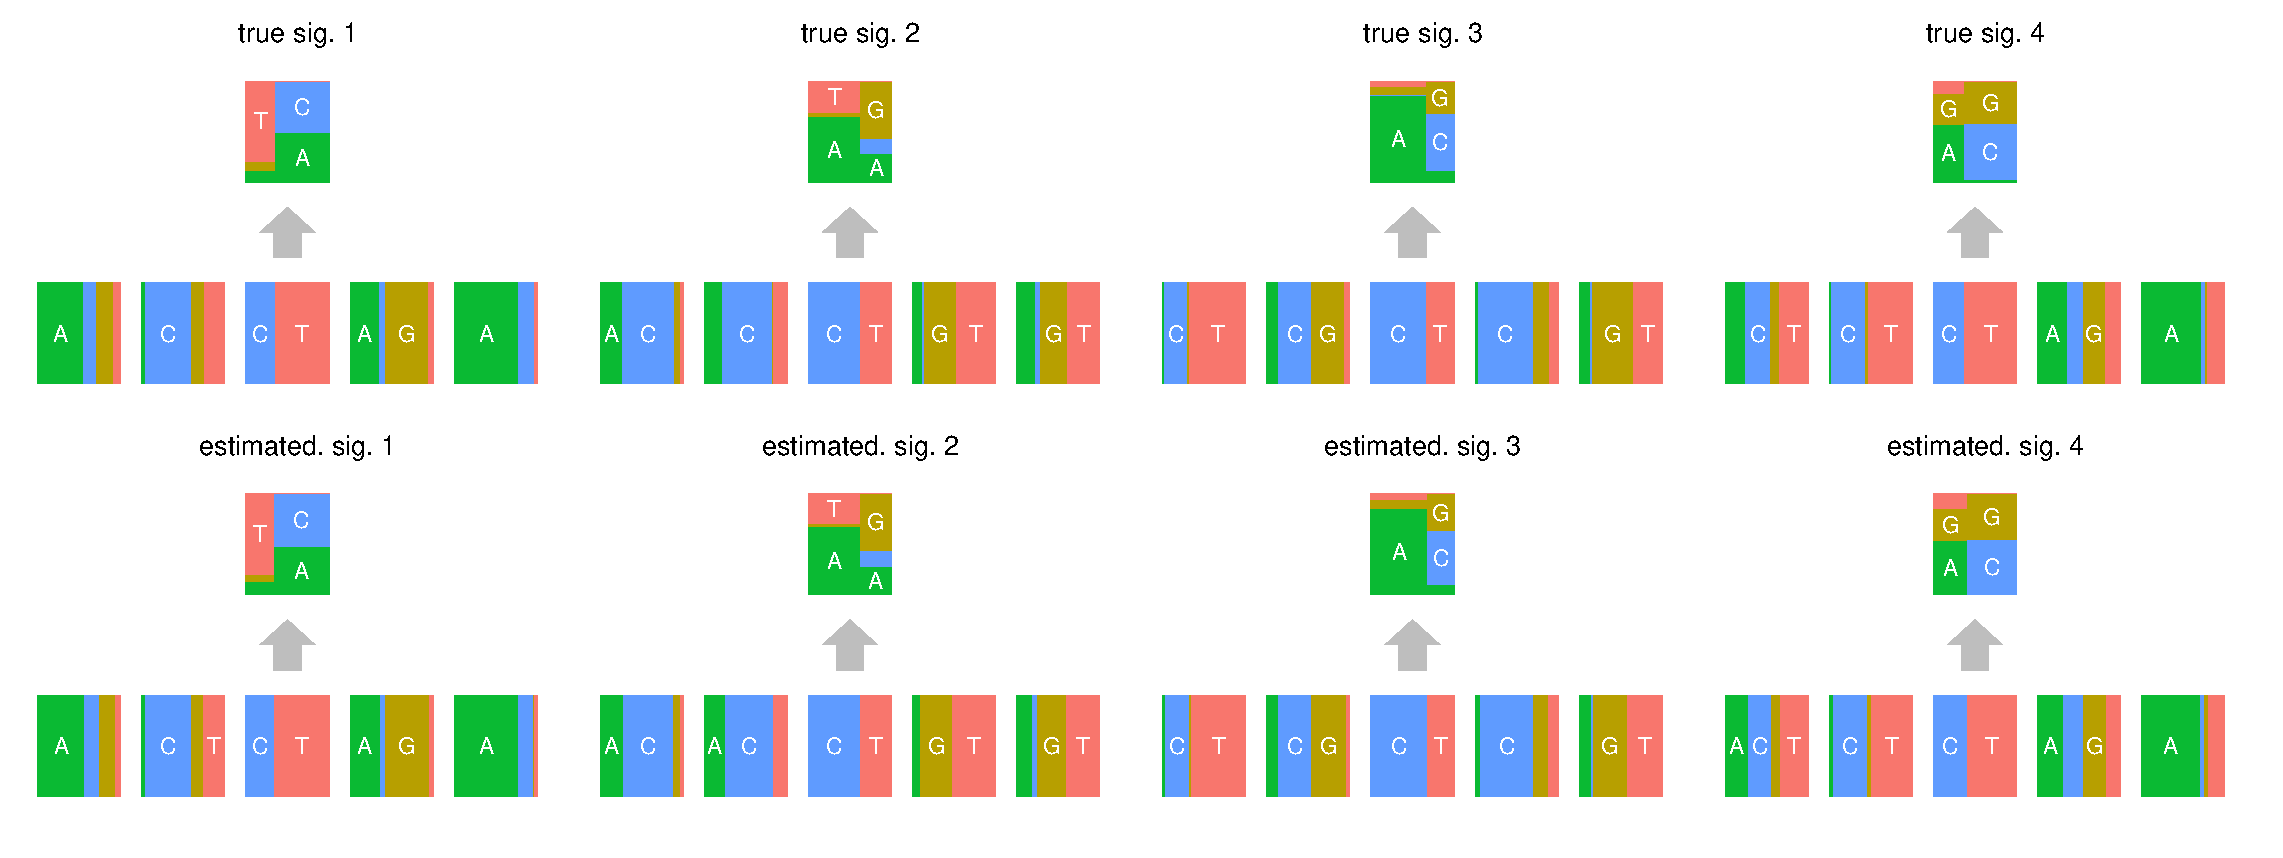
\includegraphics[width=15cm,height=5.5cm]{simulation_signature_example.eps}
\caption{An example of the relationship between true and estimated mutation signatures in the simulation.
In this example, the numbers of cancer genomes and mutations for each cancer genome are 25 and 100, respectively,
and the parameters $\alpha$ and $\gamma$ are both set to 1. 
From this figure, we can see that fairly accurate estimation is possible even with moderate numbers of cancer genomes and mutations}
\label{example_signature.pd}
\end{figure}


\clearpage

\begin{figure}
\centering
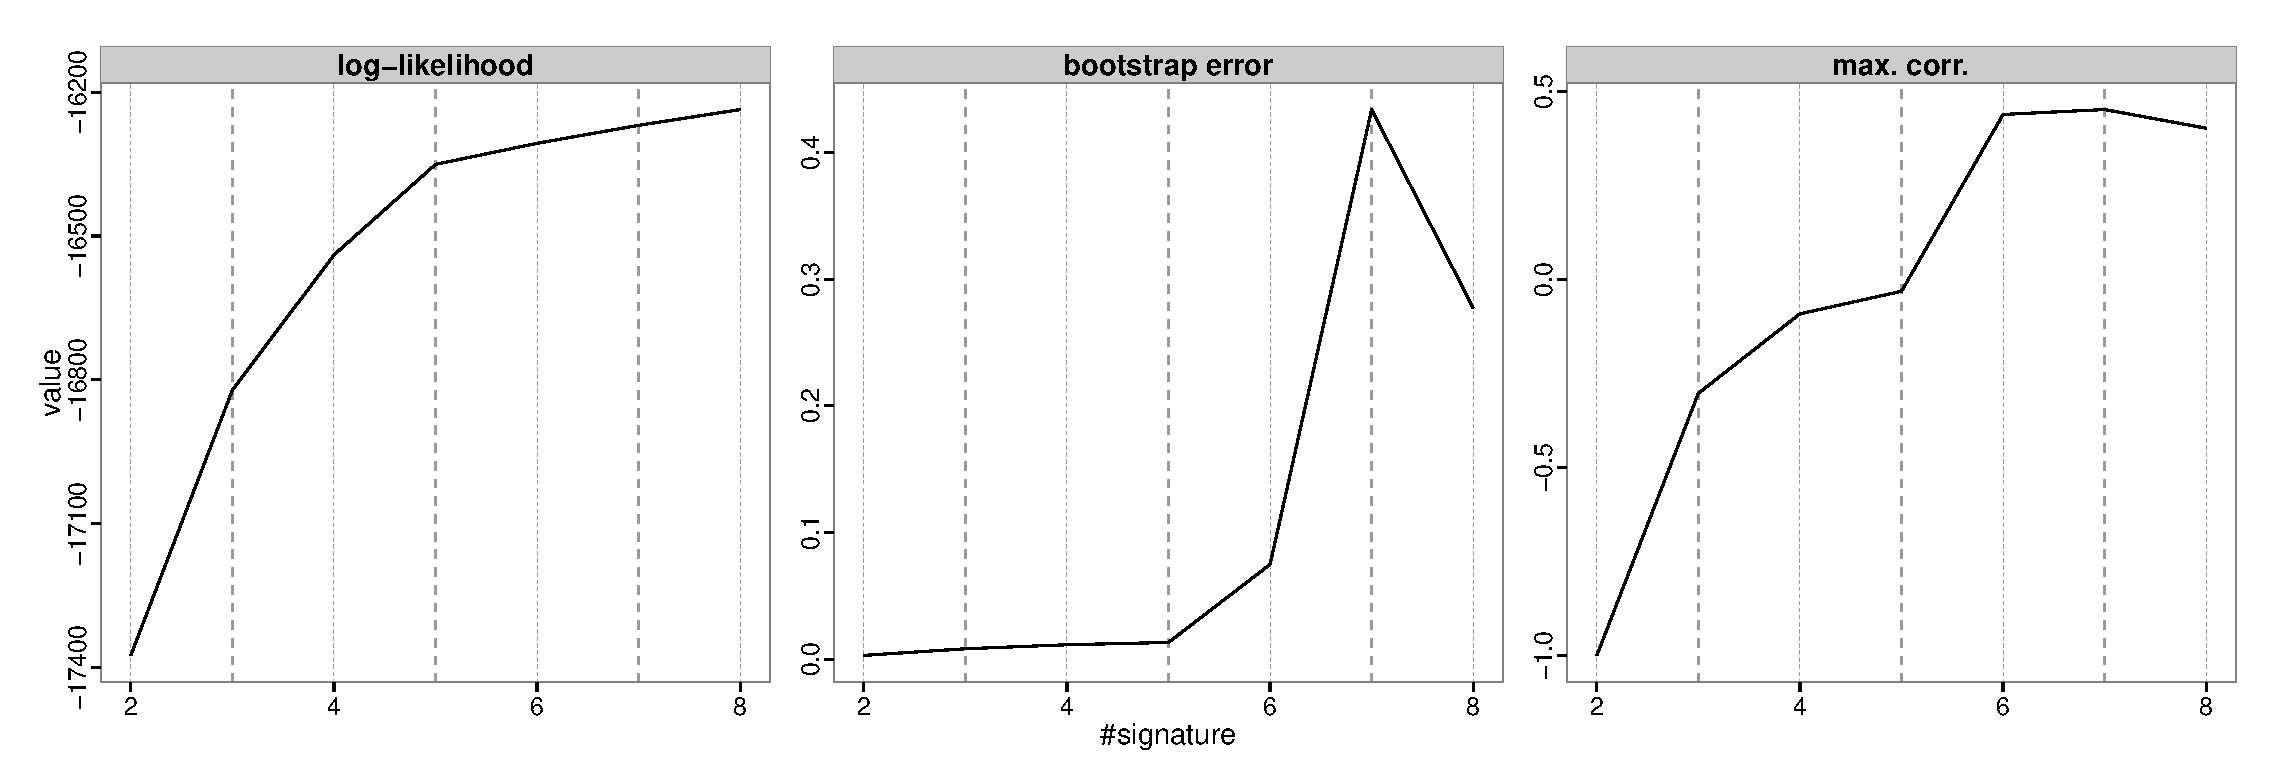
\includegraphics[width=15cm,height=5cm]{simulation_stat.eps}
\caption{The log-likelihood, bootstrap-errors and maximum correlation values among estimated membership parameters for several numbers of signatures $K$ in the trial of the Supplementary Figure 1.}
\label{example_summary.pd}
\end{figure}

\clearpage


\begin{figure}
\centering

\subfigure[$K = 2$]{%
  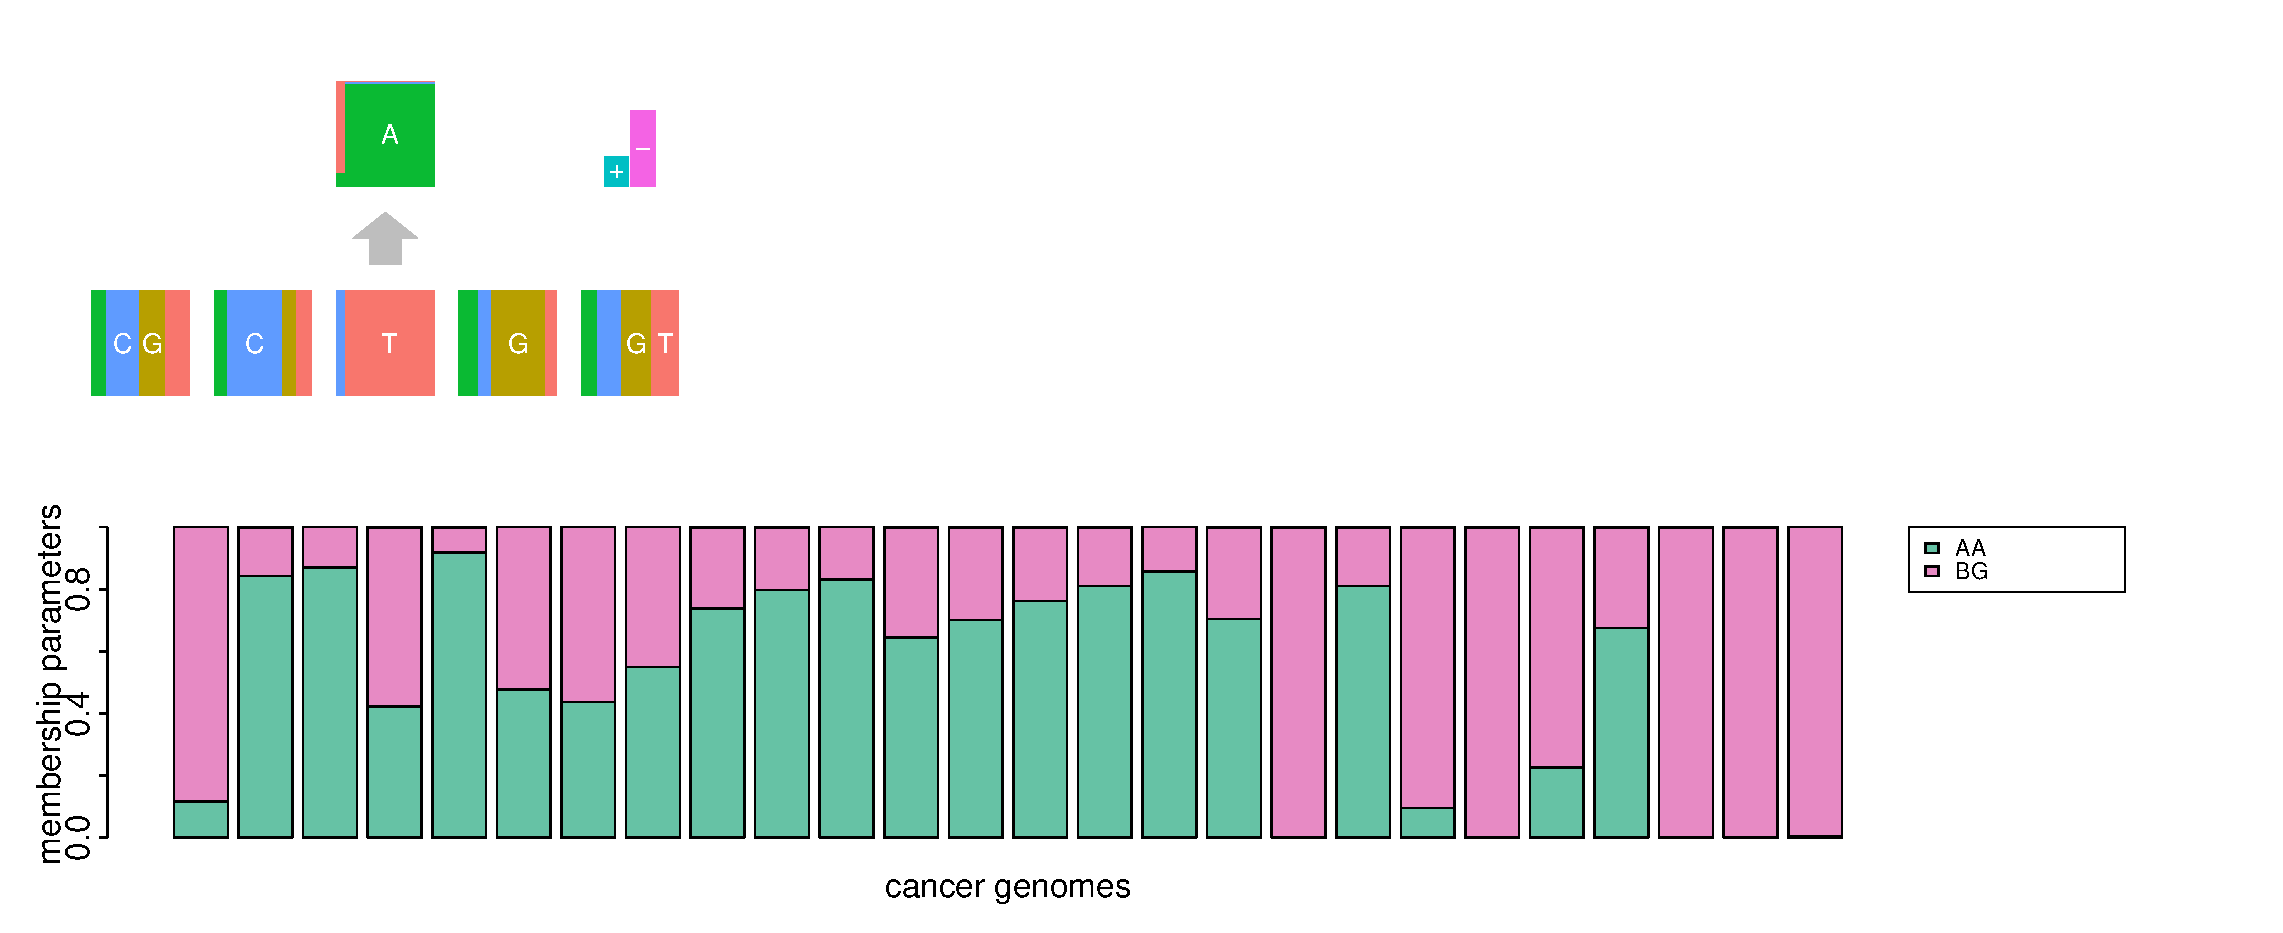
\includegraphics[height=6cm,width=15cm,clip]{UTUC_signature_K2.eps}
  \label{UTUC:sigK2_sig}}
  
  
\subfigure[$K = 3$]{%
  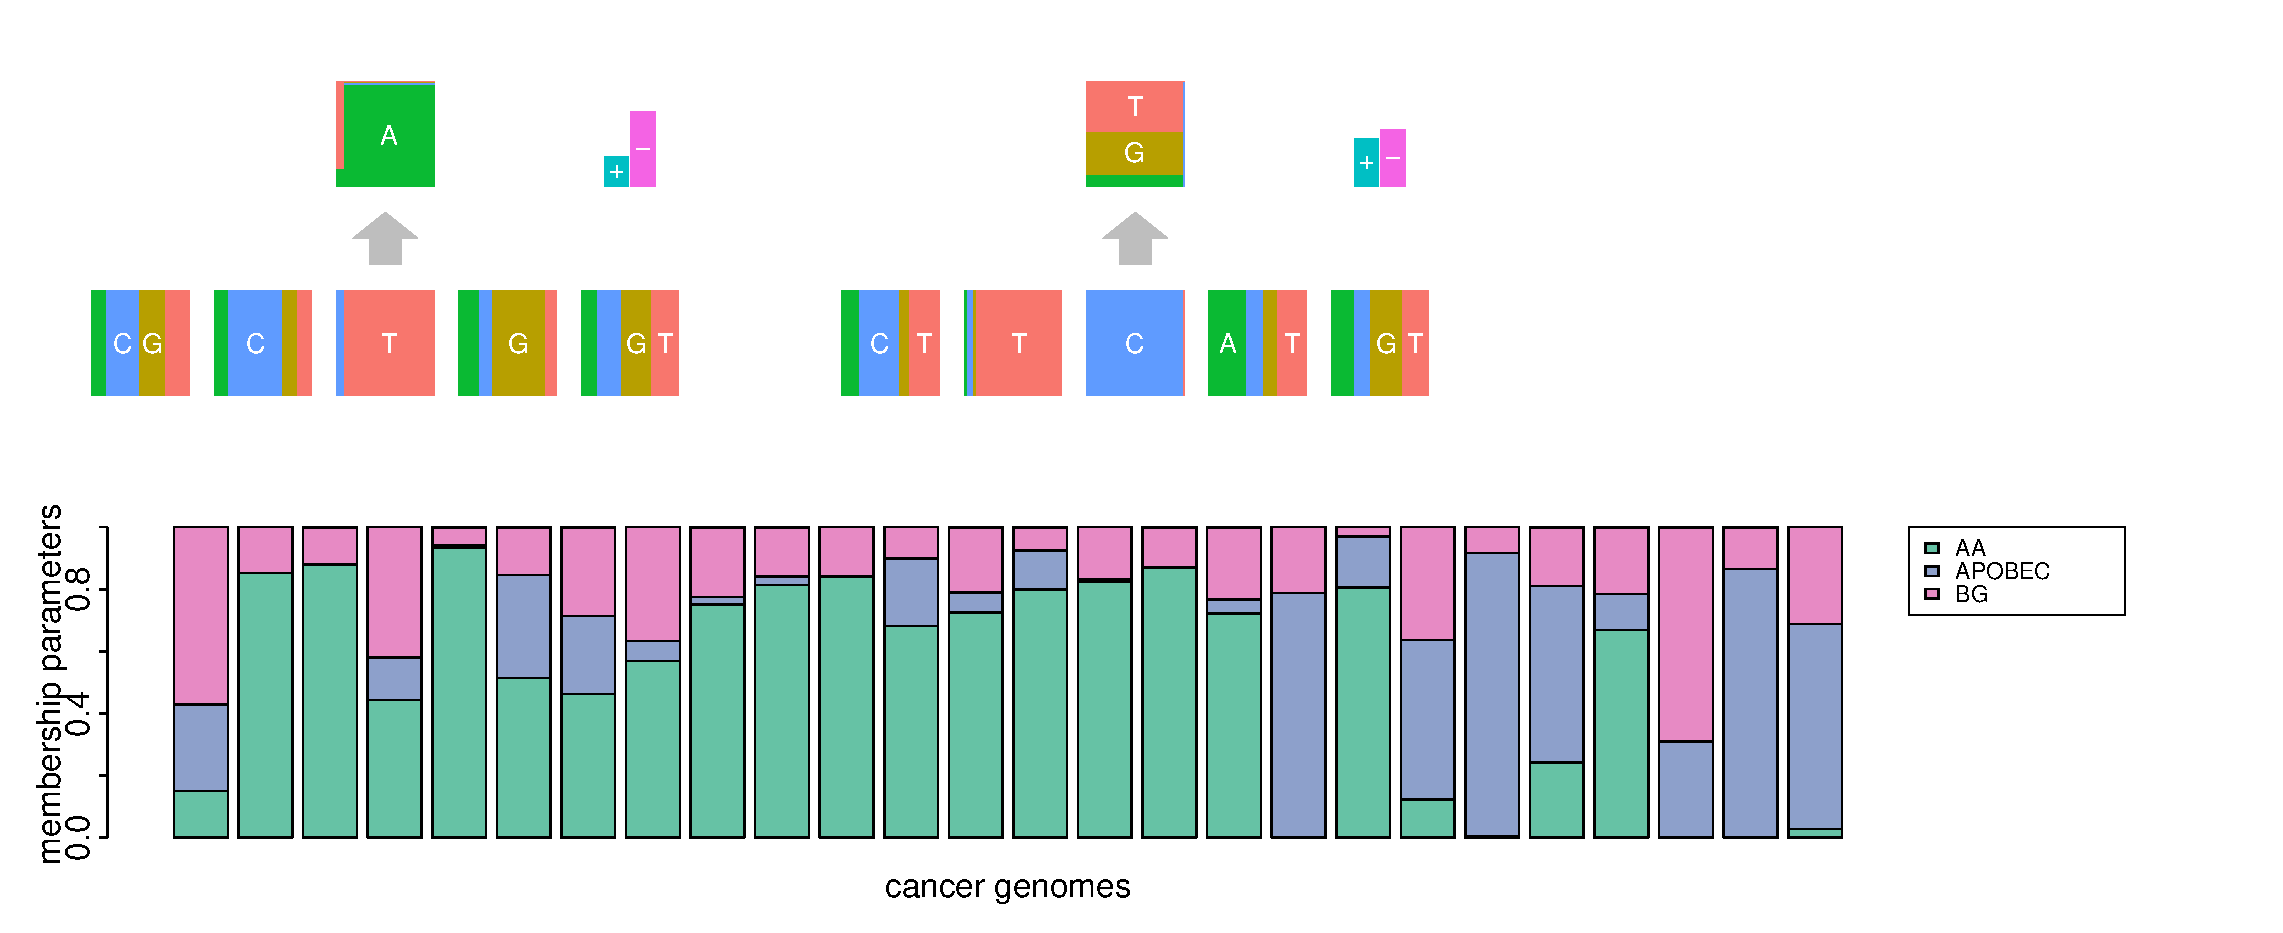
\includegraphics[height=6cm,width=15cm,clip]{UTUC_signature_K3.eps}
  \label{UTUC:sigK3_sig}}
  

\subfigure[$K = 4$]{%
  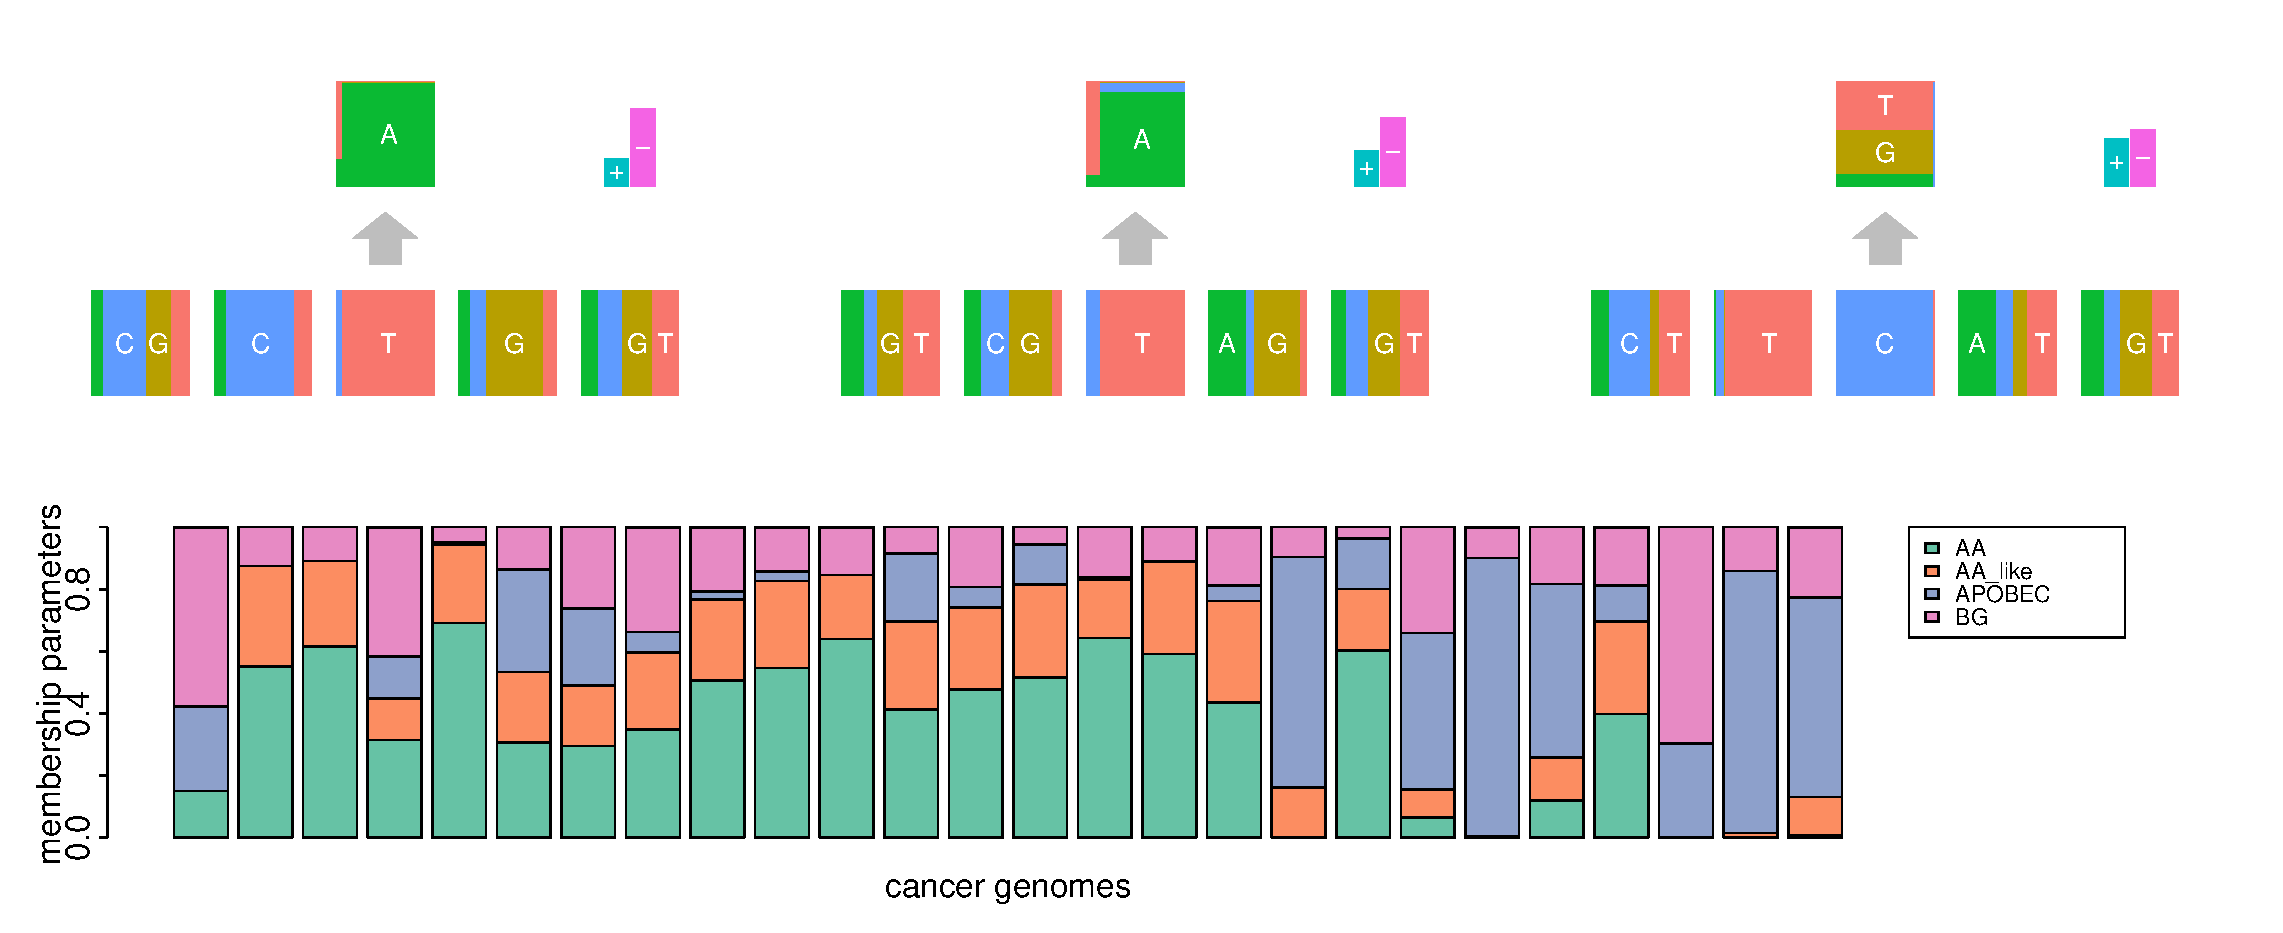
\includegraphics[height=6cm,width=15cm,clip]{UTUC_signature_K4.eps}
  \label{UTUC:sigK4_sig}}

  
\caption{The result of estimated mutation signatures and membership parameters for UTUC data 
when changing the number of mutation signatures $K$.}
\label{UTUC_multiK}
\end{figure}

\clearpage

\begin{figure}
\centering
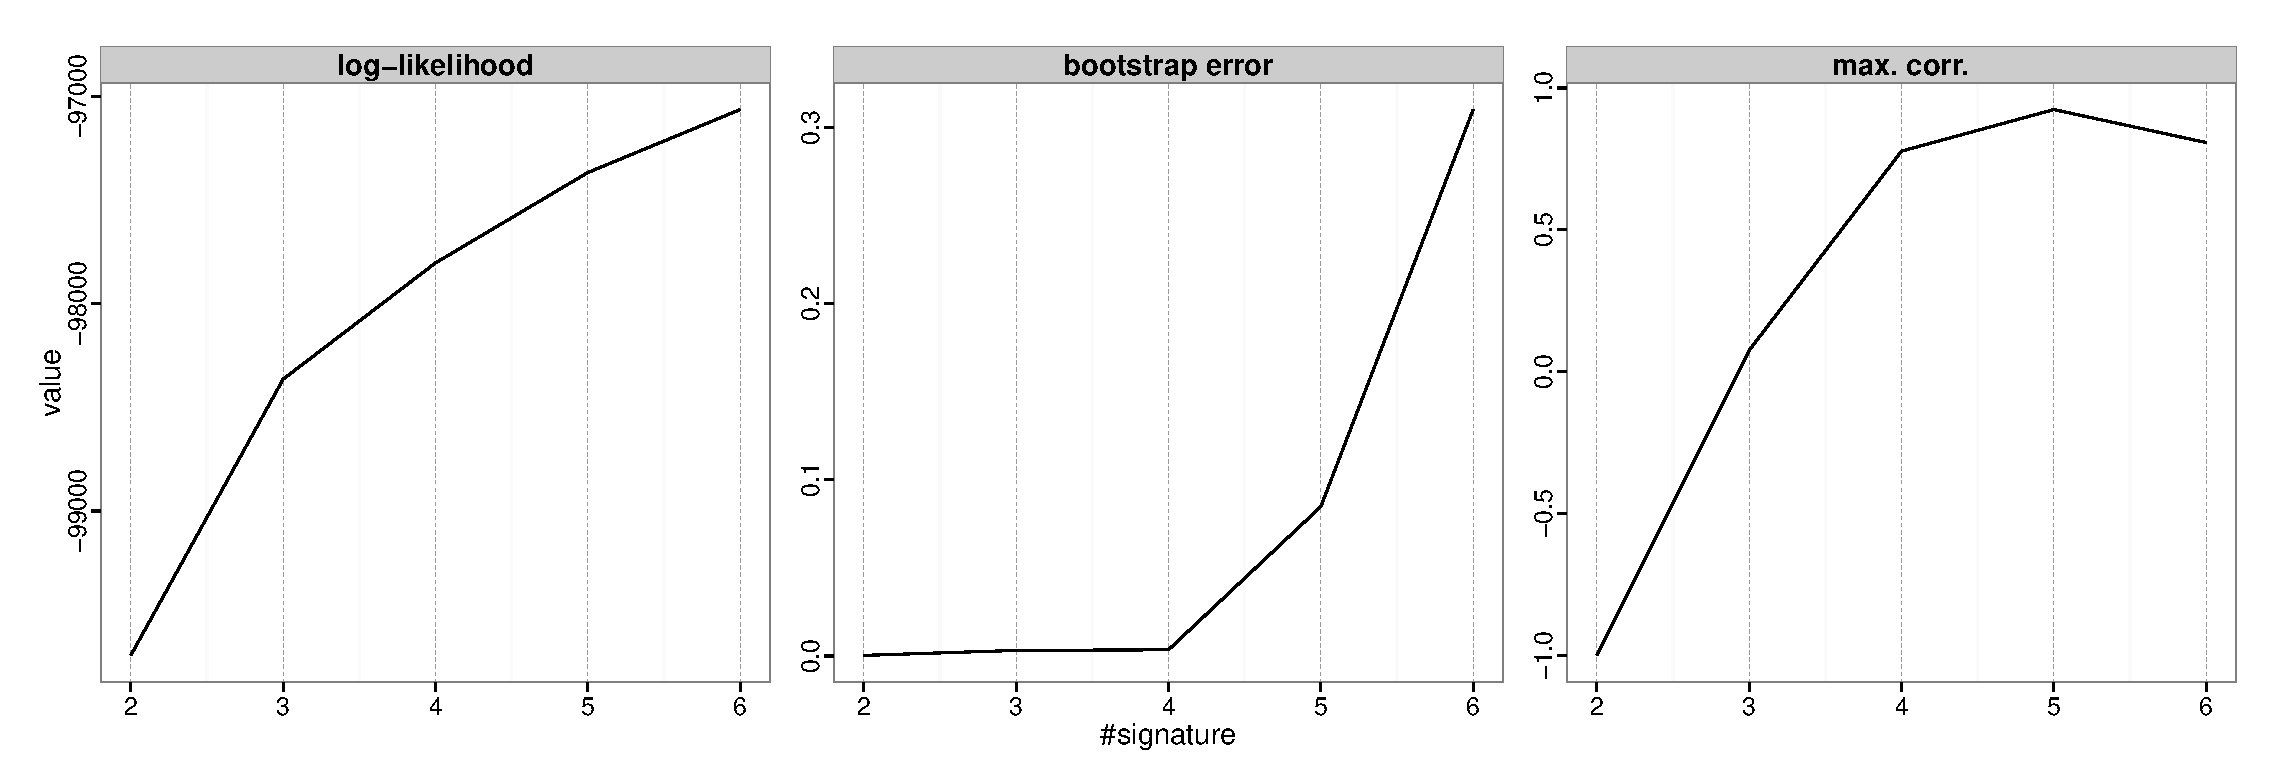
\includegraphics[width=15cm,height=5cm]{UTUC_stat.eps}
\caption{The log-likelihood, bootstrap-errors and maximum correlation values among estimated membership parameters for several numbers of signatures $K$ in UTUC data.}
\label{UTUC_stat}
\end{figure}

\clearpage

\begin{figure}
\centering
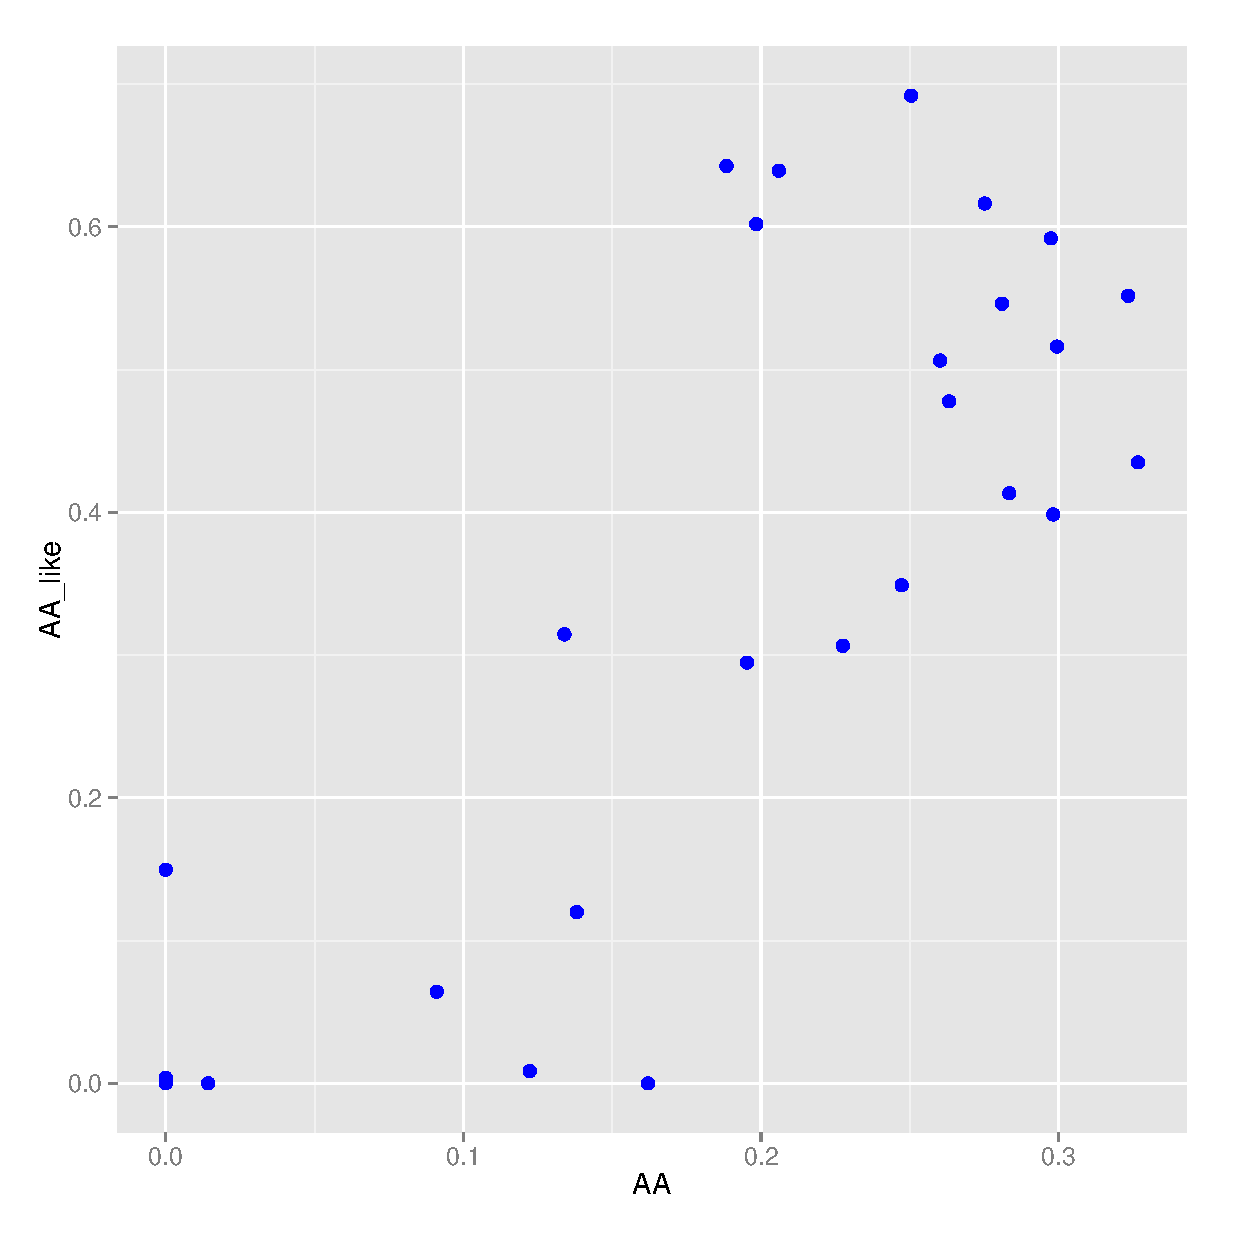
\includegraphics[width=10cm,height=10cm]{UTUC_AA_AAlike_cor.eps}
\caption{The relationships between the two membership parameters, AA (the first signature in the Supplementary Figure 3) and AA\_like (the second signature in the Supplementary Figure 3) signatures.}
\label{UTUT_AA_AAlike}
\end{figure}


\clearpage

\begin{figure}
\centering
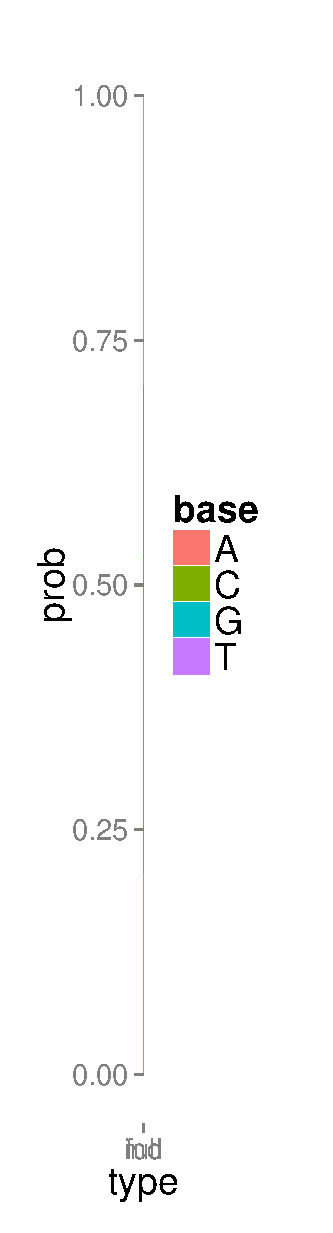
\includegraphics[width=4cm,height=8cm]{UTUC_APOBEC_twoFivePrime.eps}
\caption{The frequencies of bases at two 5' to the mutated site for the APOBEC mutation signatures obtained in UTUC data using the independent and full models.}
\label{UTUC_APOBEC_twoFivePrime}
\end{figure}


\clearpage

\begin{figure*}

\subfigure[APOBEC signature intensities at two 5' to the mutated site]{%
  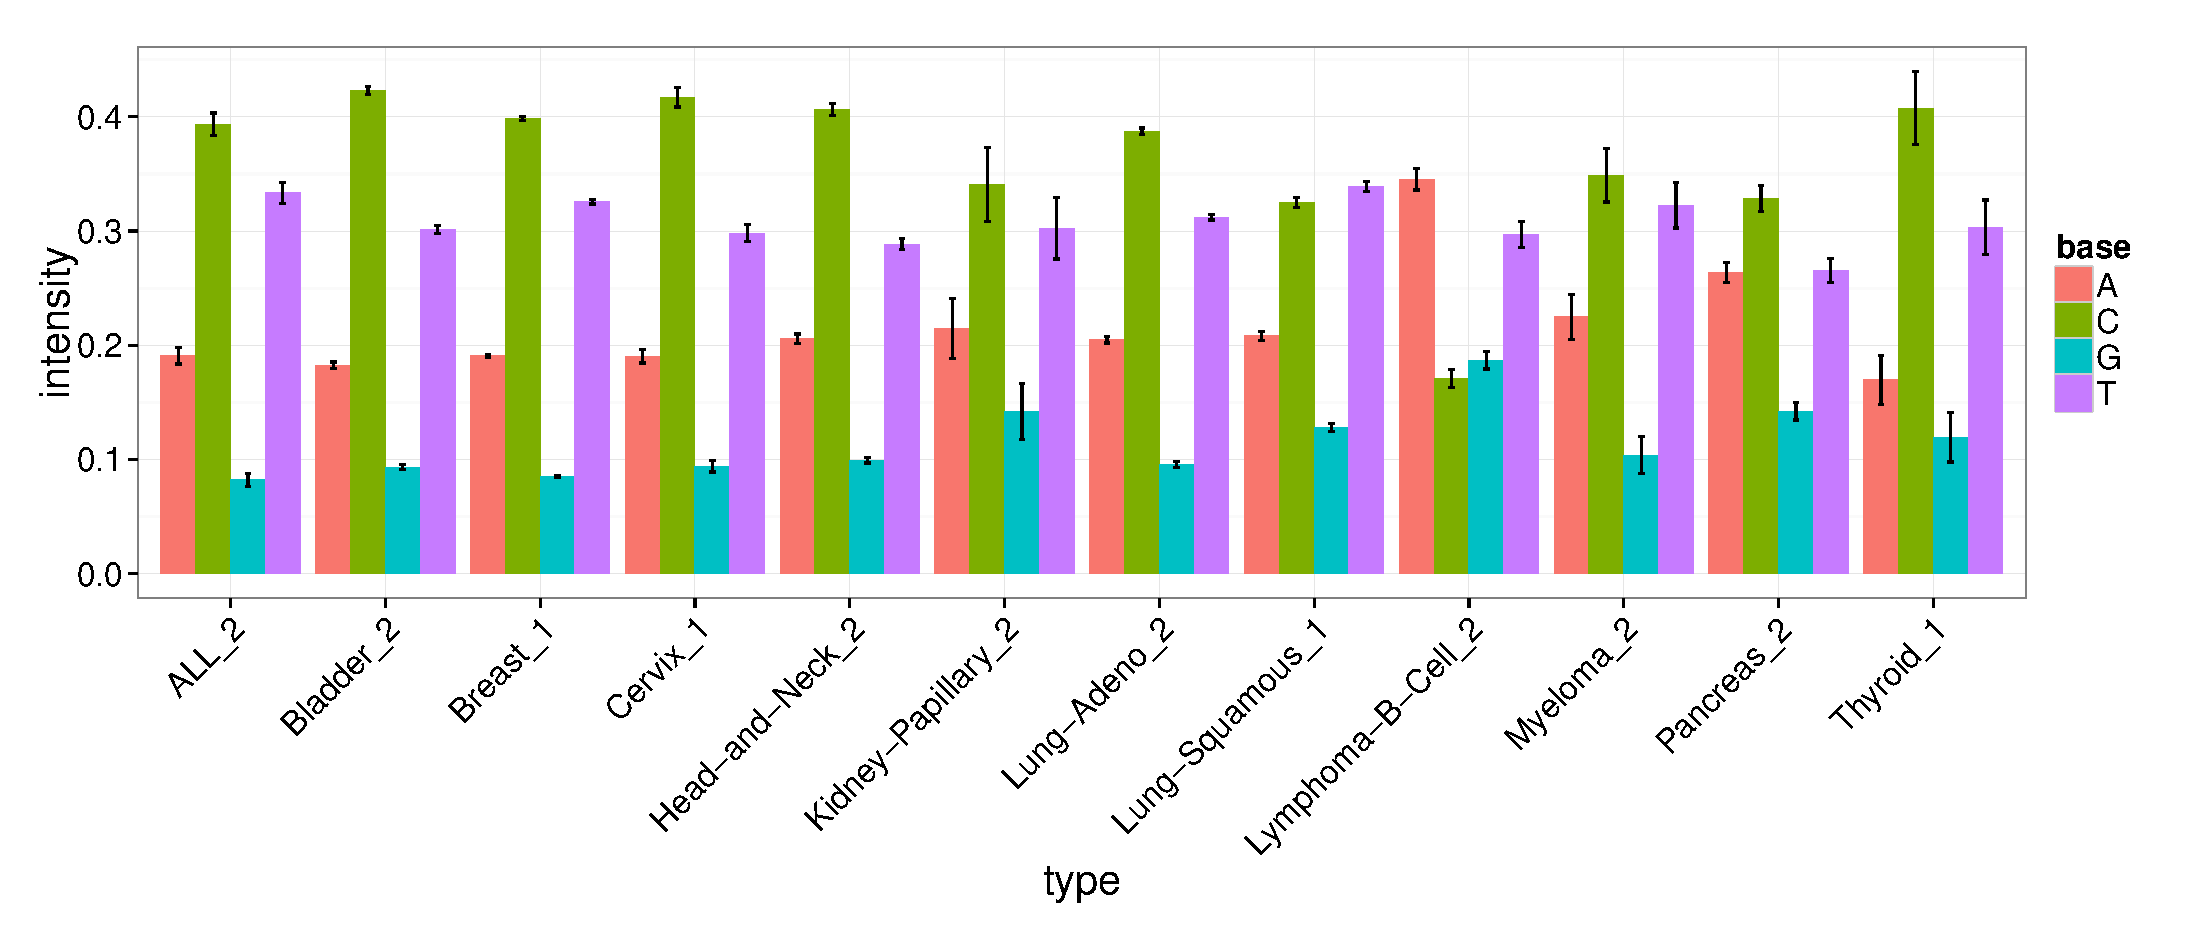
\includegraphics[width=14.5cm,height=6cm]{APOBEC_two5prime.eps}
   \label{APOBEC_two5prime}}
  
\subfigure[POLE1 signature intensities at two 5' to the mutated site]{%
  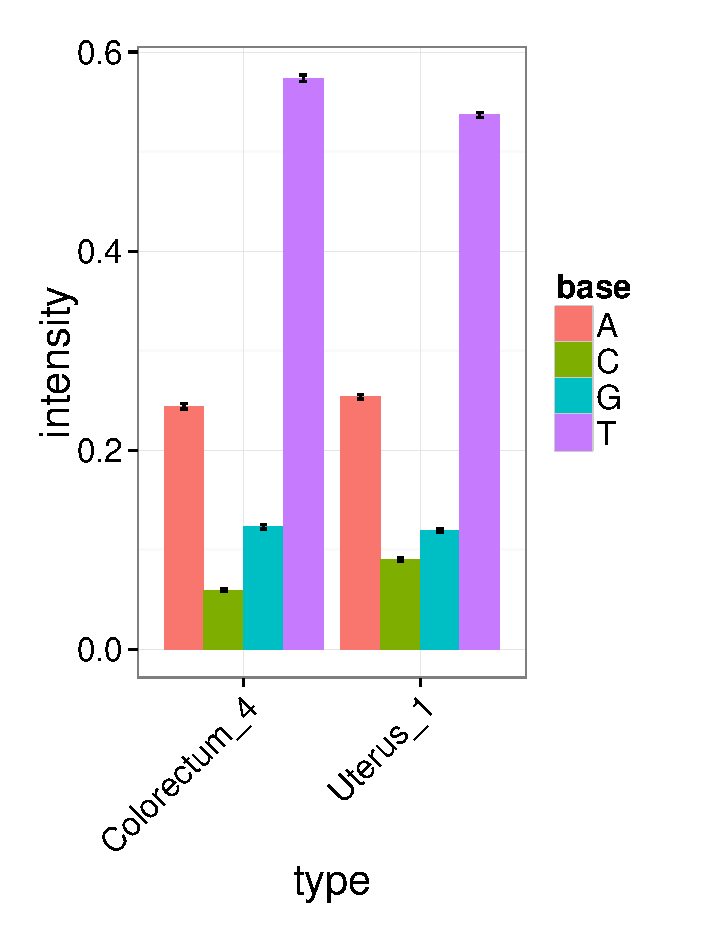
\includegraphics[width=4.5cm,height=6cm]{POLE1_two5prime.eps}
  \label{POLE1_two5prime}}
\quad
\subfigure[POLE2 signature intensities at two 5' to the mutated site]{%
  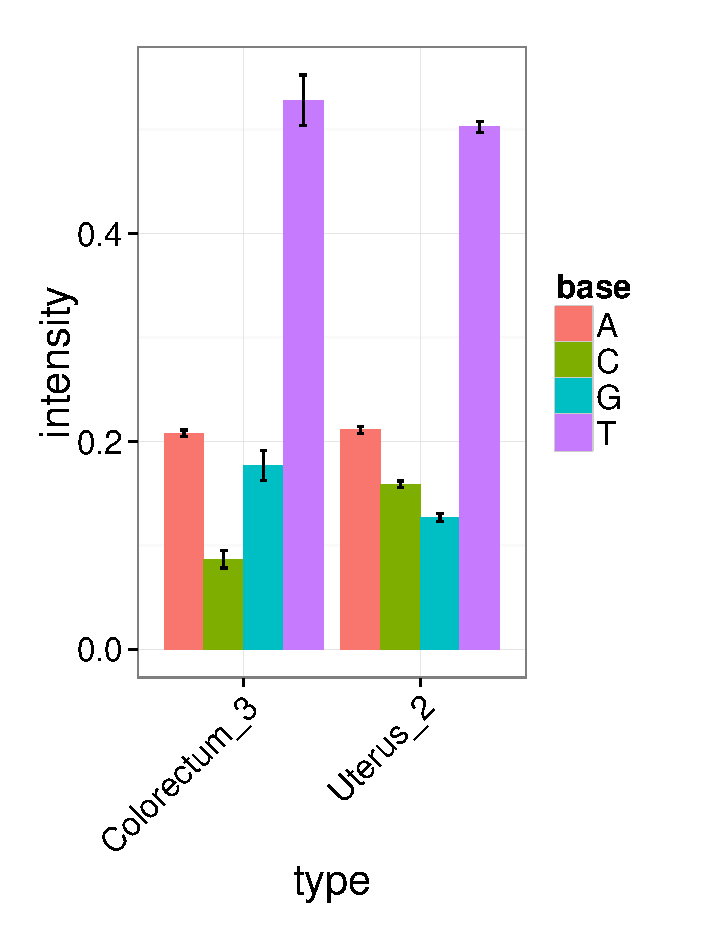
\includegraphics[width=4.5cm,height=6cm]{POLE2_two5prime.eps}
  \label{POLE2_two5prime}}

\subfigure[UV signature intensities at two 5' to the mutated site]{%
  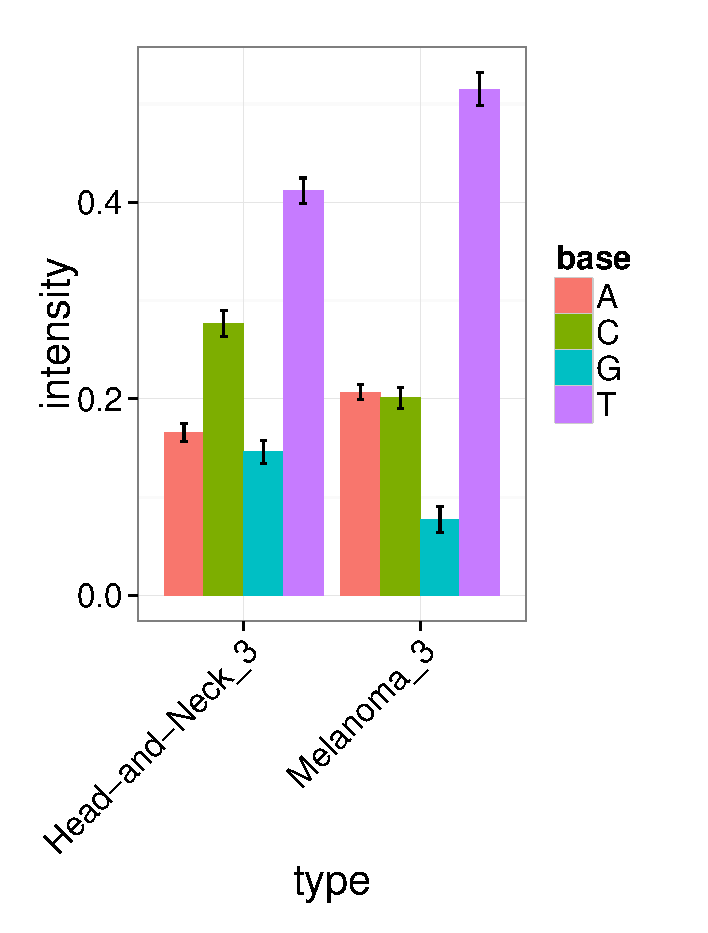
\includegraphics[width=4.5cm,height=6cm]{UV_two5prime.eps}
  \label{UV_two5prime}}
\quad
\subfigure[The signature 11 intensities at two 5' to the mutated site]{%
  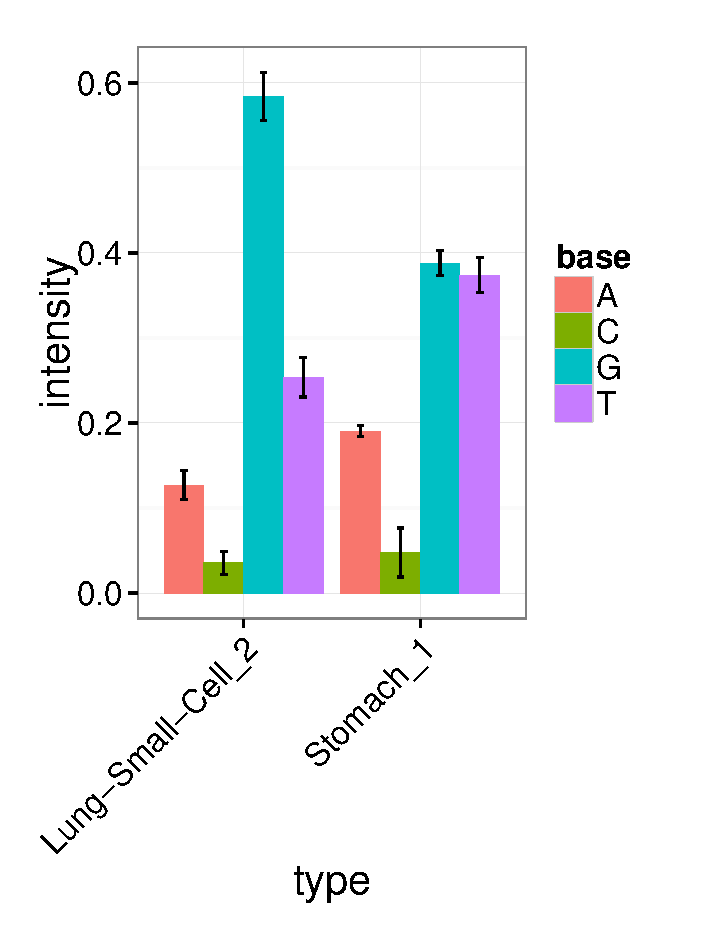
\includegraphics[width=4.5cm,height=6cm]{LMST_two5prime.eps}
  \label{LMST_two5prime}}
  
\caption{The estimated frequencies of bases at two 5' to the mutated site for each cancer type.
The heights of bar show the estimated frequency for bases A, C, G and T at two 5' to the mutated site.
The error bars show standard errors estimated by bootstrap.}
\label{two5prime}

\end{figure*}


\clearpage


\begin{figure}
\centering

\subfigure[The low grade glioma specific signature in the previous study (the ``Signature 14'' in \cite{pmid23945592})]{%
  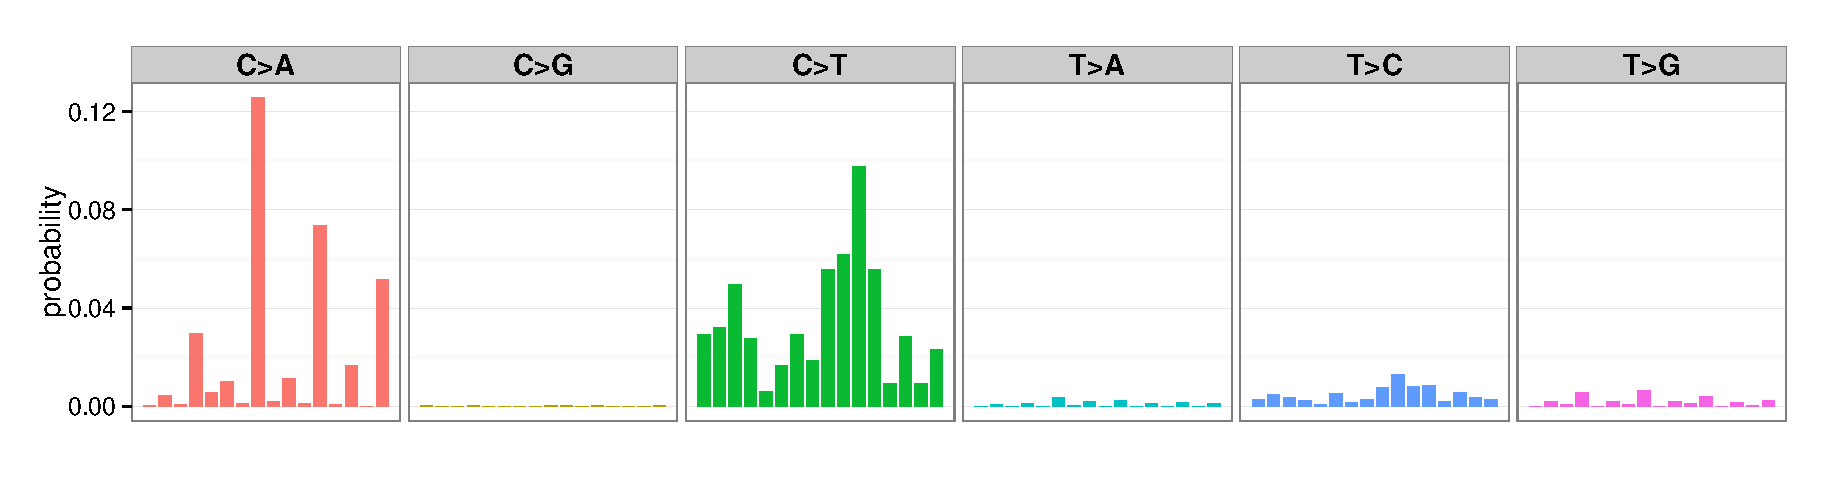
\includegraphics[height=3cm,width=12cm,clip]{example96_Glioma-Low-Grade.eps}
  \label{LGG_nature2013_sig}}
  
\subfigure[Estimated membership parameter by the proposed method]{%
  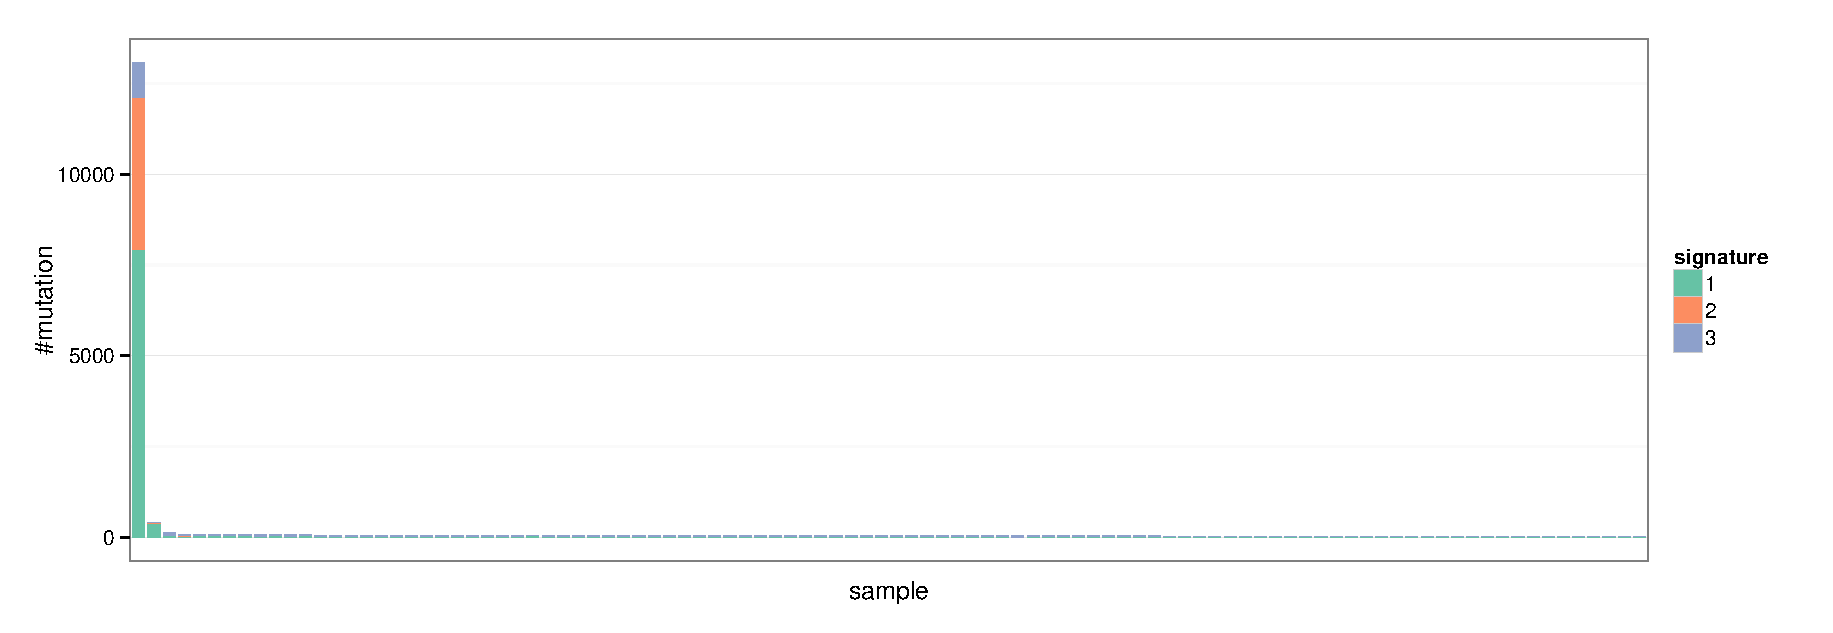
\includegraphics[height=4cm,width=12cm,clip]{Glioma-Low-Grade_membership.eps}
  \label{LGG_membership}}
\quad
\subfigure[Estimated membership parameter by the proposed method in log scale]{%
  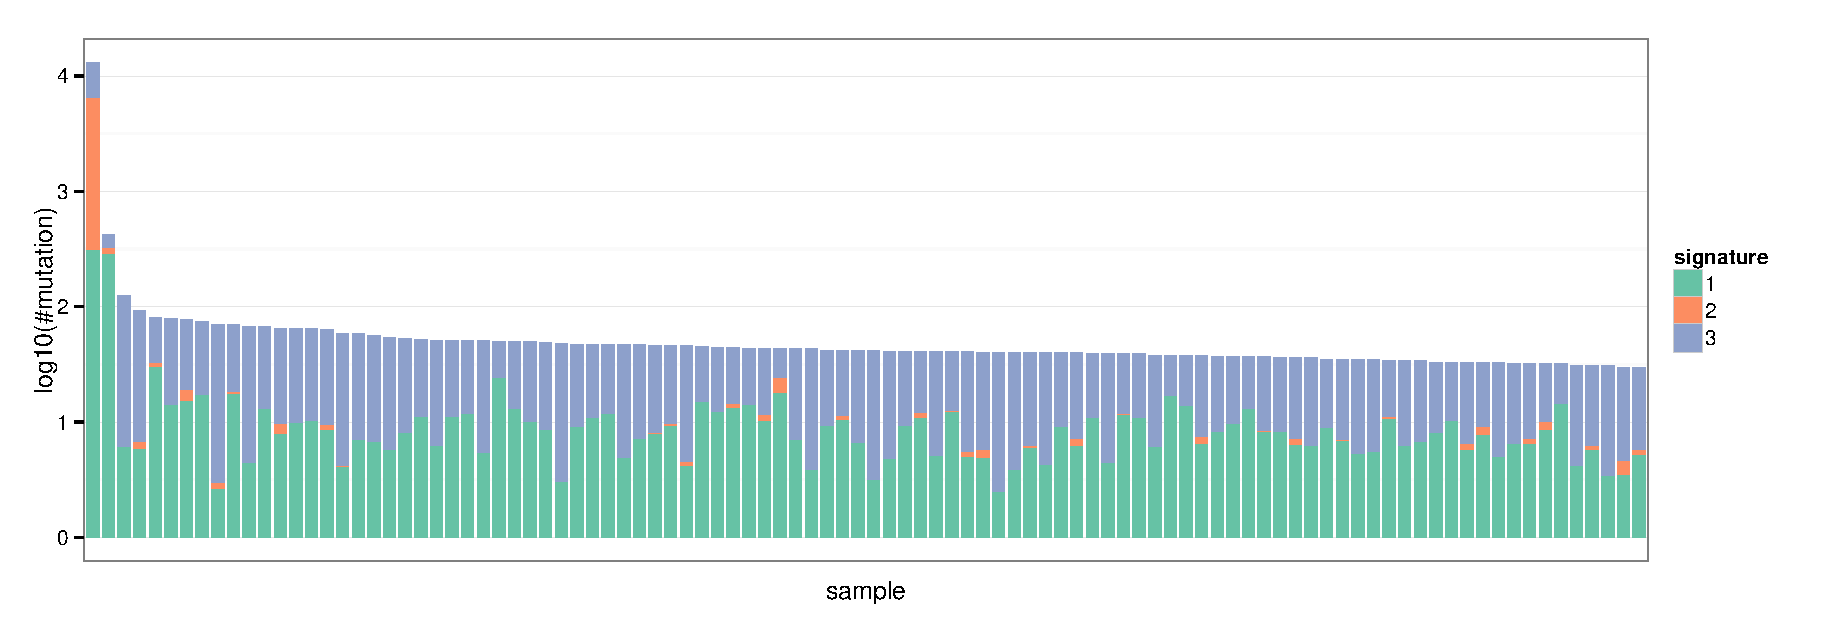
\includegraphics[height=4cm,width=12cm,clip]{Glioma-Low-Grade_membership_log.eps}
  \label{LGG_membership_log}}

  \caption{(a) The barplot is divided by 6 substitution patterns. In each division, 
16 bars show joint probabilities of 16 combinations of the immediate 5' and 3' bases.
(b, c) We have selected top 100 cancer samples according to the number of mutation.
The height of bar shows (the logarithm of) the number of mutations for each sample,
and the ratio of colored division shows the ratio of estimated membership parameters for each signature and sample.
The low grade glioma specific signature detected by the proposed method is the signature 2.
We can see that the mutations corresponding to signature 2 is mostly from the sample with an extremely high mutation rate.
}

\end{figure}

\clearpage

\begin{figure}
\centering

\subfigure[The result for the original data ($K = 2$)]{%
  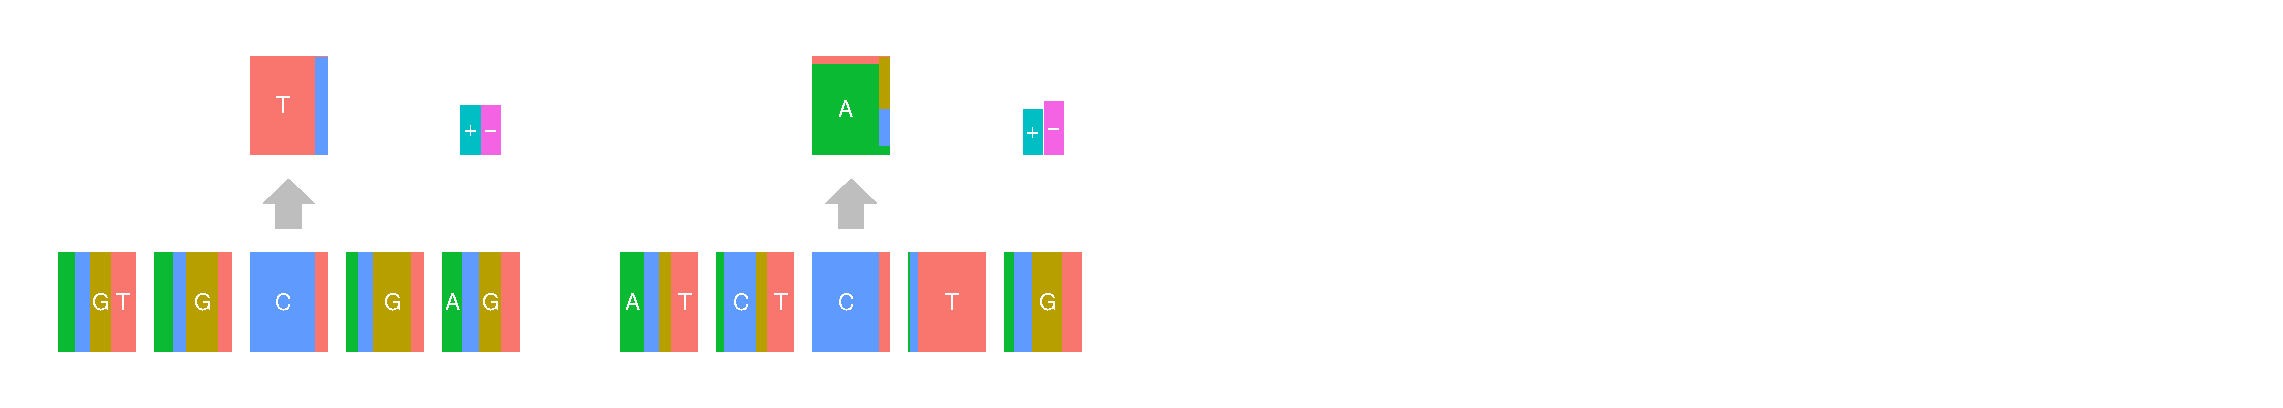
\includegraphics[height=2.5cm,width=15cm,clip]{Glioma-Low-Grade_original_signature_K2.eps}
  \label{LGG_roriginal_sigK2_sig}}
  
\subfigure[The result for the data without the hyper-mutated sample ($K = 2$)]{%
  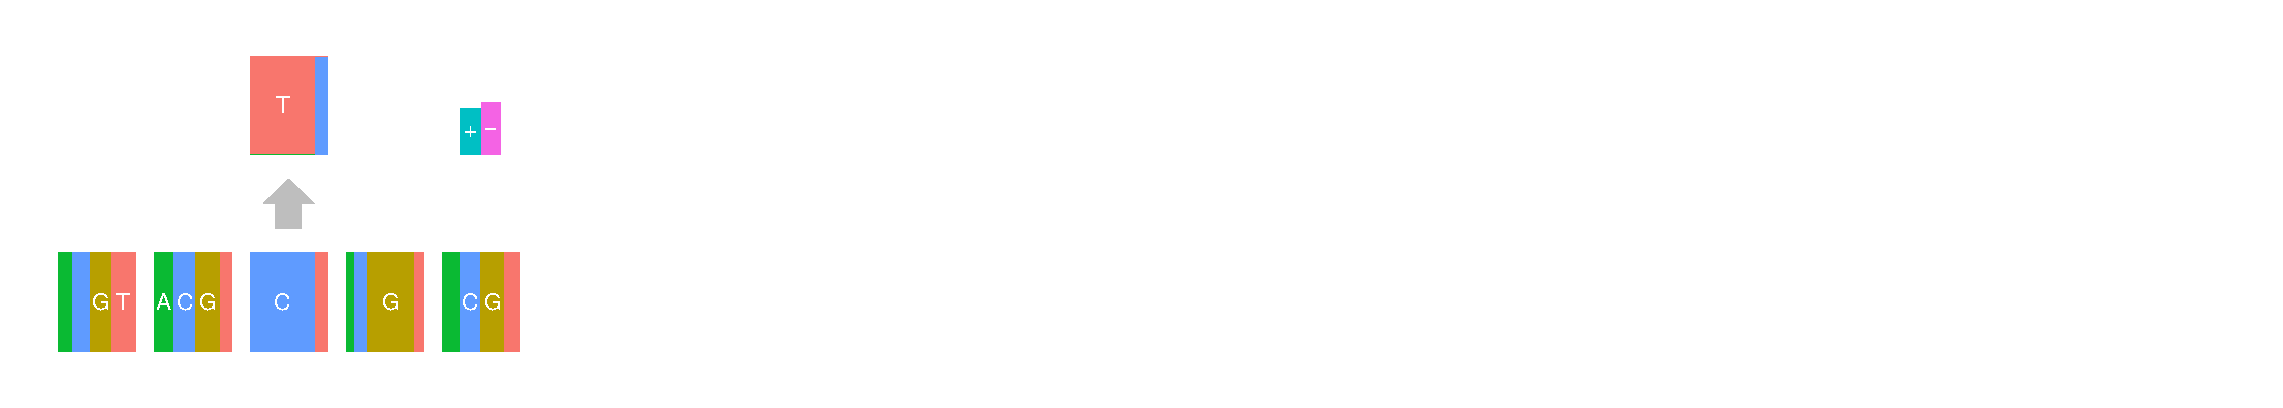
\includegraphics[height=2.5cm,width=15cm,clip]{Glioma-Low-Grade_removed_signature_K2.eps}
  \label{LGG_removed_sigK2_sig}}
  
  
\subfigure[The result for the data without the hyper-mutated sample ($K = 3$)]{%
  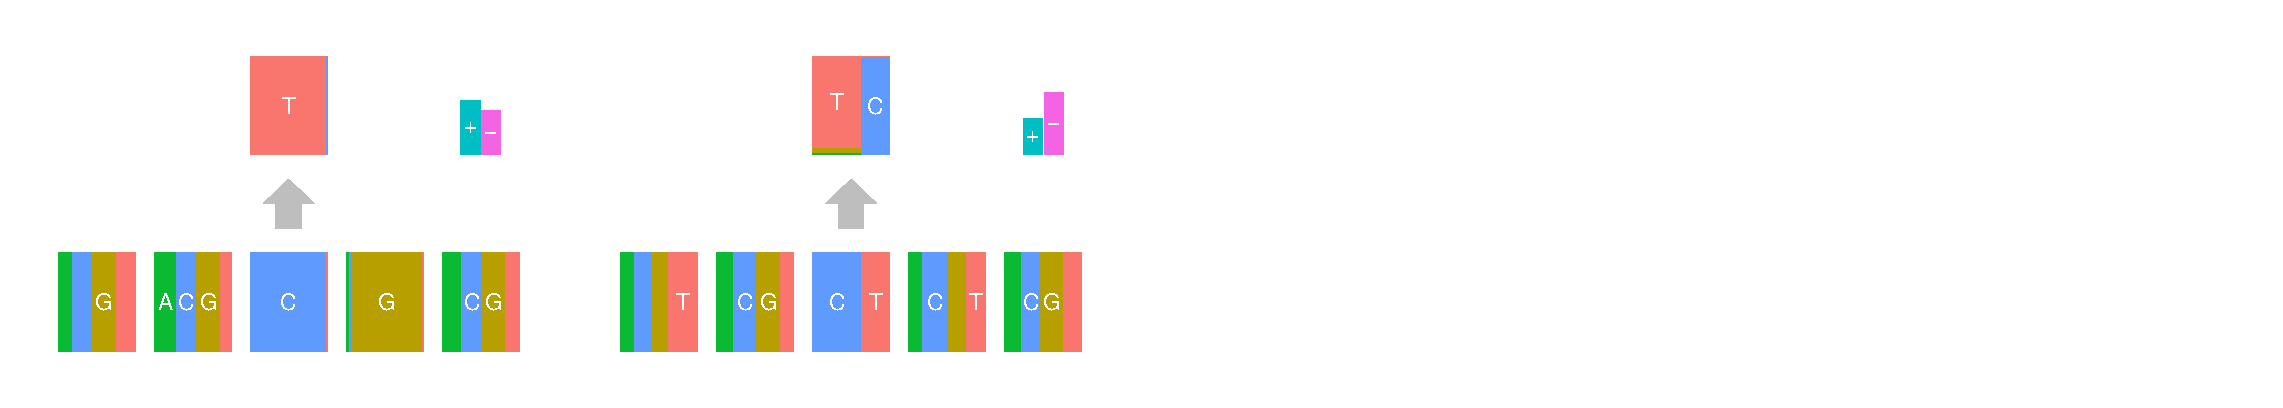
\includegraphics[height=2.5cm,width=15cm,clip]{Glioma-Low-Grade_removed_signature_K3.eps}
  \label{LGG_removed_sigK3_sig}}
  

\subfigure[The result for the data without the hyper-mutated sample ($K = 4$)]{%
  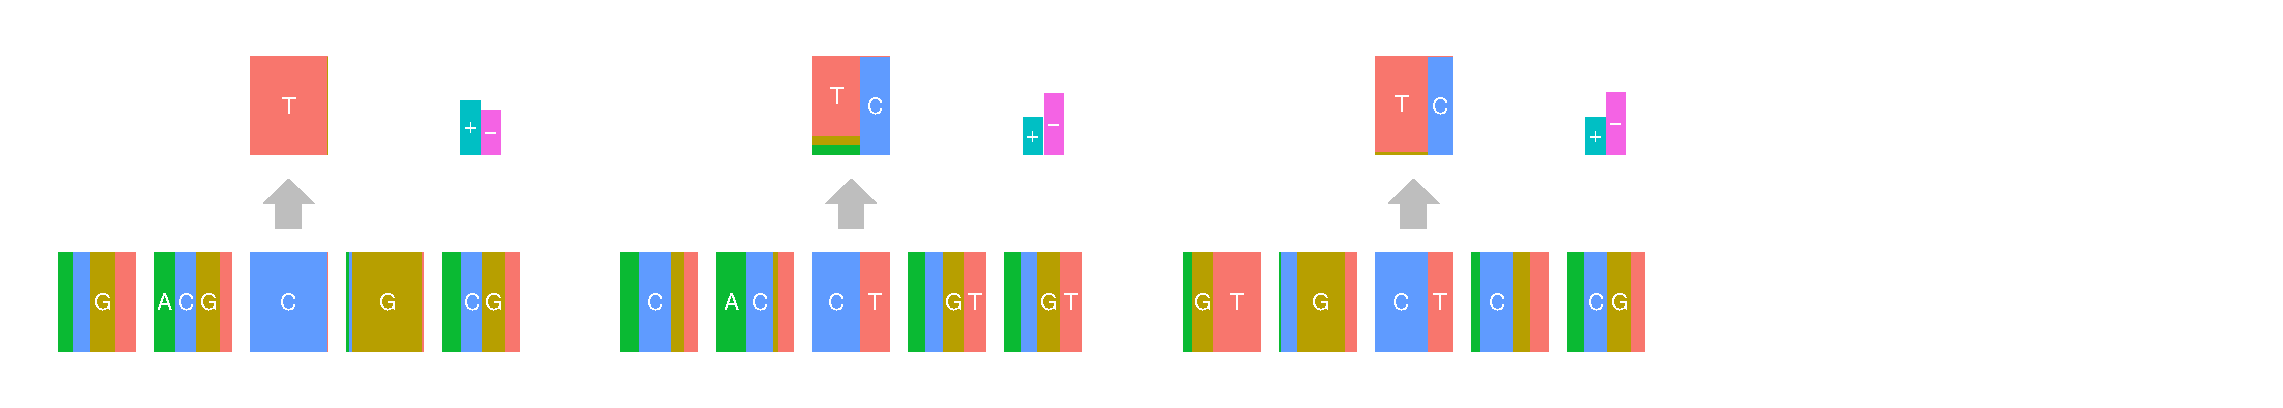
\includegraphics[height=2.5cm,width=15cm,clip]{Glioma-Low-Grade_removed_signature_K4.eps}
  \label{LGG_removed_sigK4_sig}}
  
\subfigure[The result for the data without the hyper-mutated sample ($K = 5$)]{%
  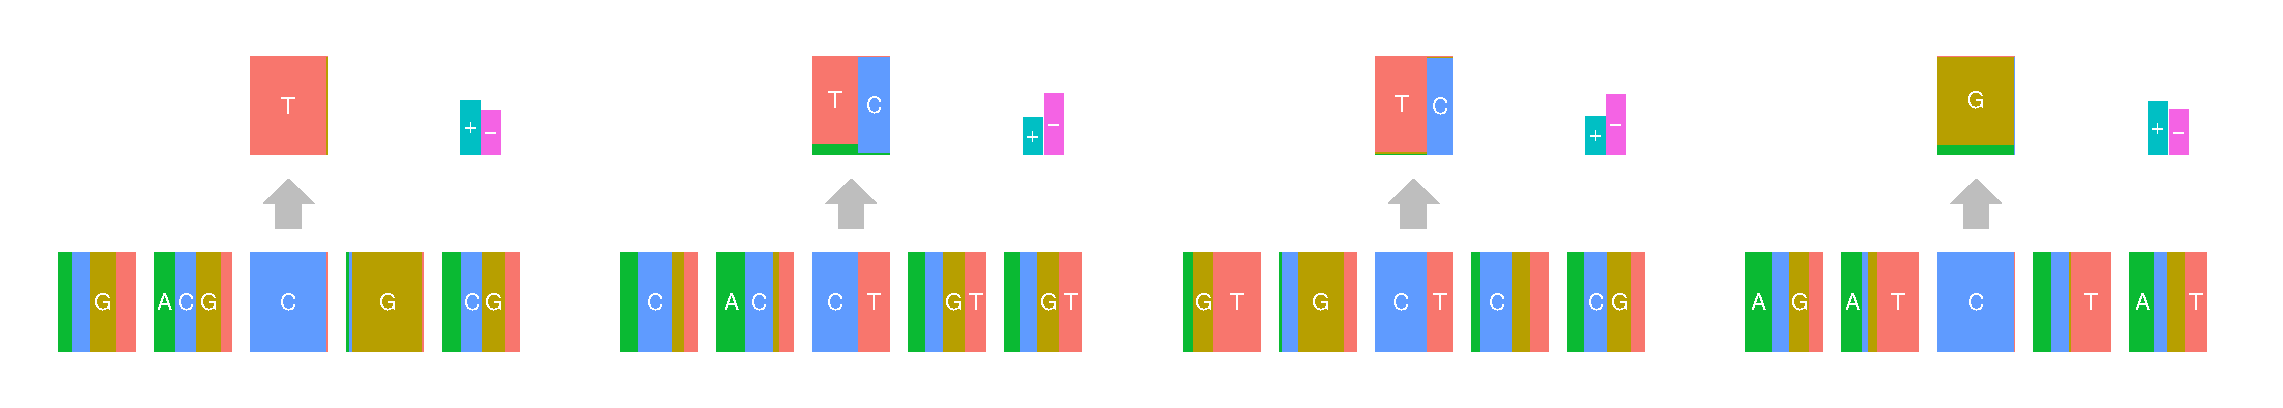
\includegraphics[height=2.5cm,width=15cm,clip]{Glioma-Low-Grade_removed_signature_K5.eps}
  \label{LGG_removed_sigK5_sig}}
  
  \caption{(a) The signatures obtained for the original data. The first (from the left) signature seems to be deamination of 5-methyl-cytosine. 
  The second signature is the low grade glioma signature. 
  (b, c, d, e) The signature obtained for the data without the hyper-mutated case for several number of mutation signatures ($K$, including the background signature).
  Although the signature related to deamination of 5-methyl-cytosine remained, low grade glioma specific signature could not be observed.}

\end{figure}

\clearpage


\begin{figure}
\centering

\subfigure[The signature 2 detected in kidney clear cell carcinomas]{%
  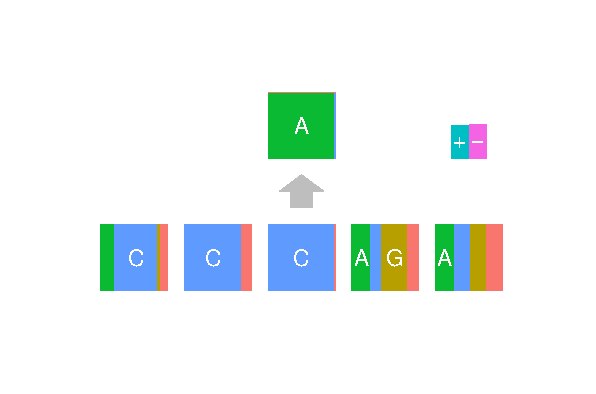
\includegraphics[height=3cm,width=4.8cm,clip]{Kidney-Clear-Cell_oxidation_signature.eps}
  \label{LGG_membership}}
\quad
\subfigure[The signature 1 detected in lung adenocarcinomas]{%
  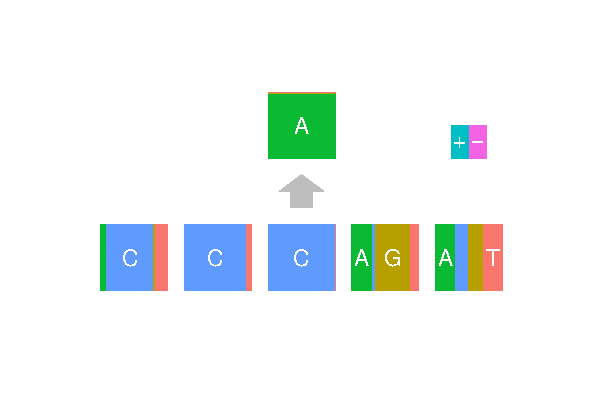
\includegraphics[height=3cm,width=4.8cm,clip]{Lung-Adeno_oxidation_signature.eps}
  \label{LGG_membership_log}}
\quad
\subfigure[The signature 1 detected in melanomas]{%
  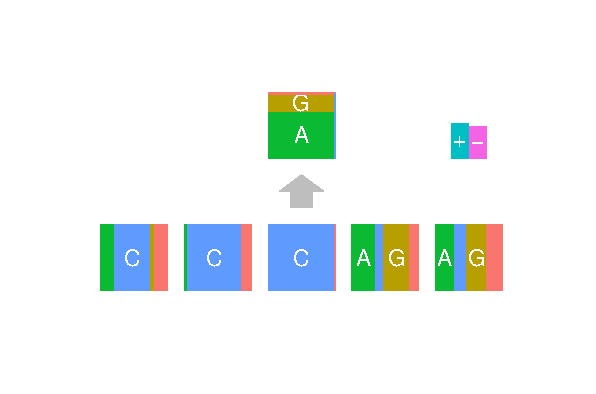
\includegraphics[height=3cm,width=4.8cm,clip]{Melanoma_oxidation_signature.eps}
  \label{LGG_membership_log}}  
  
\subfigure[Estimated membership parameter for kidney clear cell carcinomas]{%
  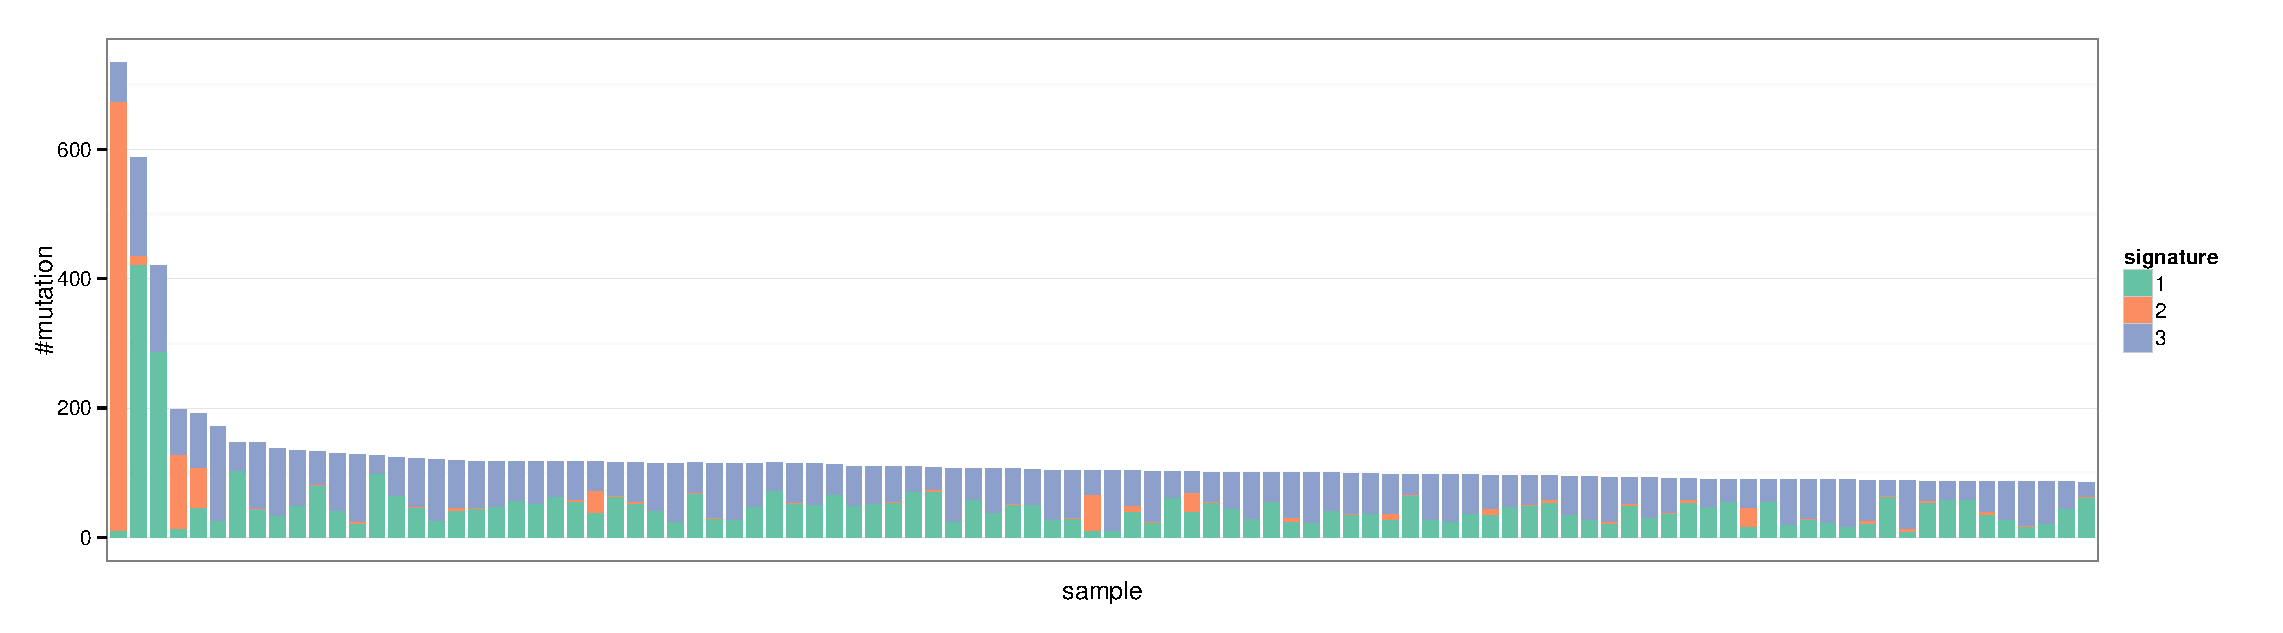
\includegraphics[height=4cm,width=12cm,clip]{Kidney-Clear-Cell_oxidation_membership.eps}
  \label{LGG_nature2013_sig}}
  
\subfigure[Estimated membership parameter for lung adenocarcinomas]{%
  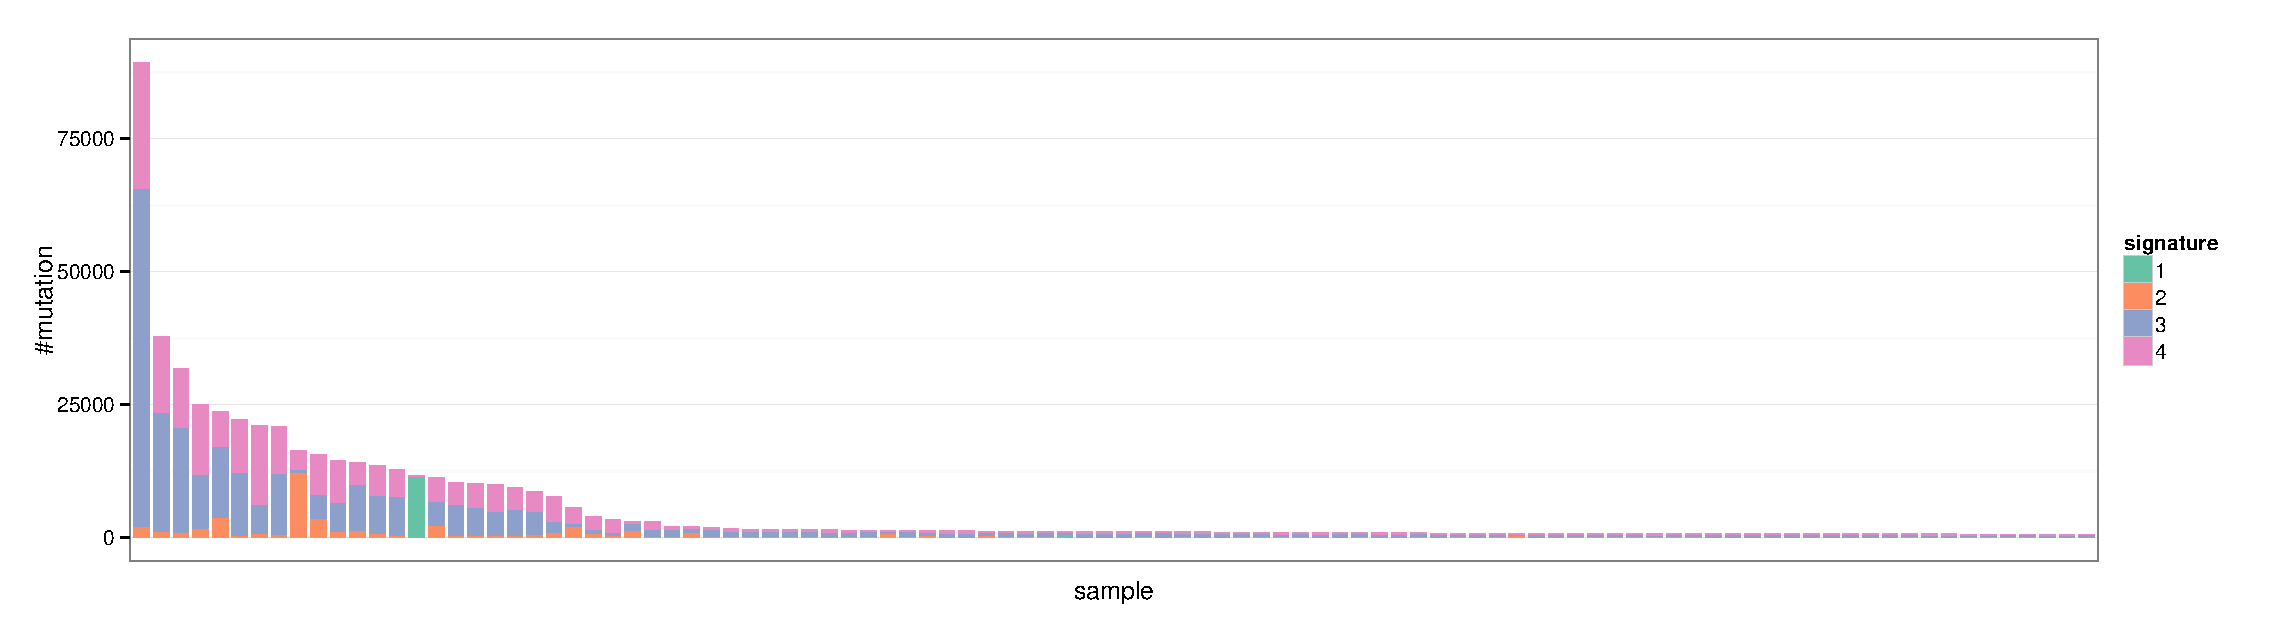
\includegraphics[height=4cm,width=12cm,clip]{Lung-Adeno_oxidation_membership.eps}
  \label{LGG_membership}}
\quad
\subfigure[Estimated membership parameter for melanomas]{%
  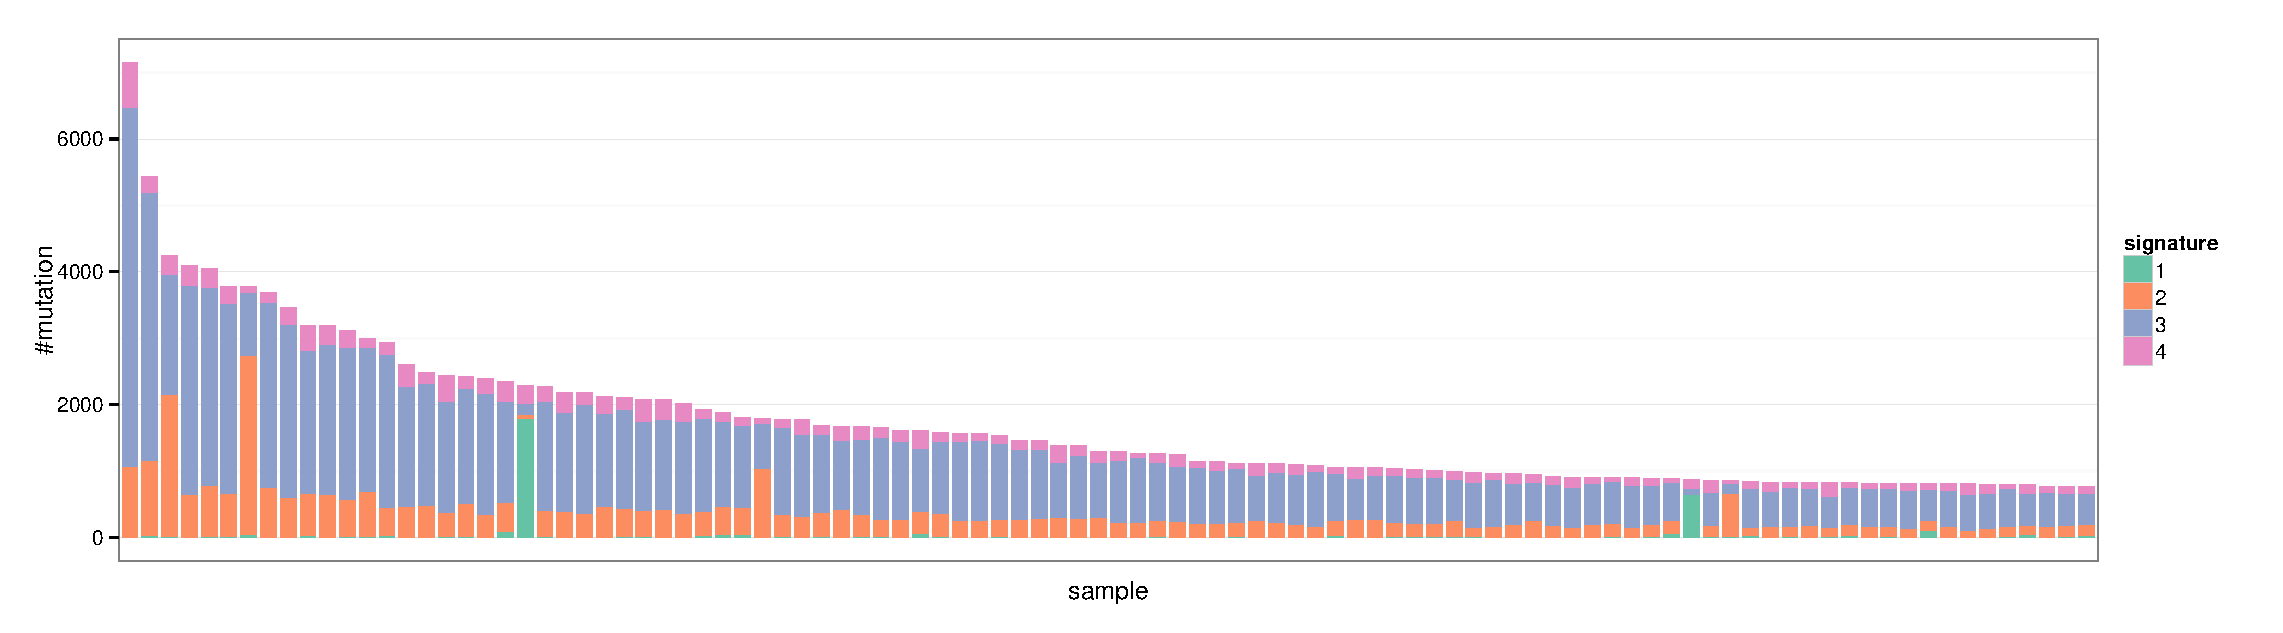
\includegraphics[height=4cm,width=12cm,clip]{Melanoma_oxidation_membership.eps}
  \label{LGG_membership_log}}

  \caption{(a, b, c) The putative oxidative artifact signatures estimated for each cancer.
  We can observe consistent abundance of the base C at the $-2 $ position.
  (d, e, f) For each cancer type, 
We have selected top 100 cancer samples according to the number of mutation.
The height of bar shows the number of mutations for each sample,
and the ratio of colored division shows the ratio of estimated membership parameters for each signature and sample.
We can see that the signature corresponding to putative oxidative artifacts concentrates on a small number of samples.}

\end{figure}



\end{document}

